%%%%%%%%%%%%%%%%%%%%%%%%%%%%%%%%%%%%%%%%%%%%%%%%%%%%%%%%%%%%%%%%%%%%%%%%%%%%%%%%
%2345678901234567890123456789012345678901234567890123456789012345678901234567890
%        1         2         3         4         5         6         7         8

\documentclass[letterpaper, 10 pt, conference]{ieeeconf}  % Comment this line out if you need a4paper

%\documentclass[a4paper, 10pt, conference]{ieeeconf}      % Use this line for a4 paper

\IEEEoverridecommandlockouts                              % This command is only needed if 
                                                          % you want to use the \thanks command

\overrideIEEEmargins                                      % Needed to meet printer requirements.

% See the \addtolength command later in the file to balance the column lengths
% on the last page of the document

% The following packages can be found on http:\\www.ctan.org
\usepackage{graphics} % for pdf, bitmapped graphics files
\usepackage{epsfig} % for postscript graphics files
\usepackage{mathptmx} % assumes new font selection scheme installed
\usepackage{times} % assumes new font selection scheme installed
\usepackage{amsmath} % assumes amsmath package installed
\usepackage{amssymb}  % assumes amsmath package installed
\pdfminorversion=4


%%%%%%%%%%%%%%%%%%%%%%%%%%%%%%%%%%%%
%my stuff
\usepackage{subfigure} 
\usepackage{latexsym,amssymb,amsmath,amsfonts}
\usepackage{fancyhdr,subfigure}
\usepackage{epsfig,psfrag,amsmath,subfigure}
\usepackage{srcltx}
\usepackage{theorem}
\usepackage{verbatim}
\usepackage[svgnames]{xcolor} 
\usepackage{algorithm}
\usepackage[noend]{algorithmic}
\usepackage[hidelinks]{hyperref}
\usepackage{tabularx}

\newcommand{\theHalgorithm}{\arabic{algorithm}}

\theoremstyle{plain} \theorembodyfont{\upshape}
\newtheorem{theorem}{\indent Theorem}
\newtheorem{prop}[theorem]{\indent Proposition}
\newtheorem{corollary}[theorem]{\indent Corollary}
\newtheorem{definition}{\indent Definition}
\newtheorem{fact}[theorem]{\indent Fact}
\newtheorem{lemma}{\indent Lemma}
\newtheorem{assumption}{\indent Assumption}
\newtheorem{condition}{\indent Condition}
\newtheorem{remark}{\indent Remark}
\newtheorem{problem}{\indent Problem}



\newif\ifPDF \ifx\pdfoutput\undefined \PDFfalse \else \ifnum \pdfoutput > 0 \PDFtrue \else\PDFfalse \fi \fi

%\newcommand{\qed}{\nobreak \ifvmode \relax \else
%      \ifdim\lastskip<1.5em \hskip-\lastskip
%      \hskip1.5em plus0em minus0.05em \fi \nobreak
%      \vrule height0.25em width0.5em depth0.25em\fi}

\newcommand{\bea}{\begin{eqnarray}}
\newcommand{\eea}{\end{eqnarray}}
\newcommand{\be}{\begin{equation}}
\newcommand{\ee}{\end{equation}}
\newcommand{\bi}{\begin{itemize}}
\newcommand{\ei}{\end{itemize}}
%\newcommand{\XX}{{\bf XX}} %\XX
\newcommand{\nn}{{\nonumber}}
\newcommand{\motiv}{{\bf Why, How, Who cares?}}
\newcommand{\mean}{{\bf E}}
\newcommand{\meanw}{{\bf E}_w}
\newcommand{\boldp}{\bf P}
\newcommand{\boldsp}{\bf p}
\newcommand{\cov}{{\bf \Sigma}}
\newcommand{\maxmu}{{\max_\mu}}
\newcommand{\maxtmu}{{\max_{\tilde{\mu}}}}
\newcommand{\tmu}{\tilde{\mu}}
\newcommand{\hmu}{\hat{\mu}}
\newcommand{\mui}{\mu^i}
\newcommand{\mukki}{\mu^i_{k|k}}
\newcommand{\mukkj}{\mu^j_{k|k}}
\newcommand{\mukpki}{\mu^i_{k+1|k}}
\newcommand{\mukpkpi}{\mu^i_{k+1|k+1}}

\newcommand{\tPi}{\tilde{\Pi}}
\newcommand{\tpi}{\tilde{\pi}}
\newcommand{\tLambda}{\tilde{\Lambda}}
\newcommand{\hatxk}{\hat{x}_{k|k}}
\newcommand{\hatxkk}{\hat{x}_{k+1|k+1}}
\newcommand{\hatxkki}{\hat{x}_{k+1|k+1}^i}
\newcommand{\hatxki}{\hat{x}_{k|k}^i}
\newcommand{\Pk}{P_{k|k}}
\newcommand{\Pkk}{P_{k+1|k+1}}
\newcommand{\Pki}{P_{k|k}^i}
\newcommand{\Pkki}{P_{k+1|k+1}^i}

\usepackage{multirow}
%\newtheorem{thm}{Theorem}%[section]
%\newtheorem{define}[thm]{Definition}
%\newtheorem{prop}[thm]{Proposition}
%\newtheorem{lem}[thm]{Lemma}

% matrix
\newcommand{\bbm}{\begin{bmatrix}}
\newcommand{\ebm}{\end{bmatrix}}

% itemize
%\newcommand{\bi}{\begin{itemize}}
%\newcommand{\ei}{\end{itemize}}

% enumerate
\newcommand{\ben}{\begin{enumerate}}
\newcommand{\een}{\end{enumerate}}

% equationarray

% equation
\newcommand{\bes}{\begin{eqnarray*}}
\newcommand{\ees}{\end{eqnarray*}}

% indent
\newcommand{\nid}{\noindent}

% figure
\newcommand{\bfig}{\begin{figure}}
\newcommand{\efig}{\end{figure}}

% center
\newcommand{\bc}{\begin{center}}
\newcommand{\ec}{\end{center}}

% bullet
\newcommand{\nb}{\noindent $\bullet$\hspace{1.5mm}}

% ignore
\newcommand{\ignore}[1]{}

% spaces
\newcommand{\hs}[1]{\hspace{#1mm}}
\newcommand{\vs}[1]{\vspace{#1mm}}

% lists / enumerations
\newcommand{\beni}[2]
{\begin{enumerate}\setlength{\itemsep}{#1mm}\setlength{\parskip}{#2mm}}

\newcommand{\bii}[2]
{\begin{itemize}\setlength{\itemsep}{#1mm}\setlength{\parskip}{#2mm}}

\usepackage[normalem]{ulem}
% comments
\definecolor{darkgreen}{rgb}{0,0.5,0}
\definecolor{darkred}{rgb}{220,20,60}
\newcommand{\XX}[1]{\color{red}{\bf XX$>$ #1 $<$XX}\color{black}}
\newcommand{\todo}[1]{\marginpar{\raggedright \footnotesize \color{red} #1}}
\newcommand{\gXX}[1]{\color{blue}{\bf XX$>$ #1 $<$XX}\color{black}}
\newcommand{\rXX}[1]{\color{darkgreen}{\bf XX$>$ #1 $<$XX}\color{black}}
\newcommand{\tXX}[1]{\color{cyan}{\bf XX$>$ #1 $<$XX}\color{black}}
\newcommand{\gcmargin}[2]{{\color{blue}#1}\marginpar{\color{blue}\tiny\raggedright \bf [GC] #2}}
\newcommand{\gsout}[2]{{\sout{#1}}{{\gXX{#2}}}} 
\newcommand{\al}{\alpha}
\newcommand{\e}{\epsilon}
\newcommand{\la}{\lambda}
\newcommand{\s}{\sigma}
\newcommand{\p}{\partial}
\newcommand{\R}{\mathbb{R}}
\newcommand{\E}{\mathbb{E}}
\newcommand{\tr}{\mathrm{tr}}
\newcommand{\LI}{\mathcal{L}}
\newcommand{\C}{\mathcal{C}}
\newcommand{\F}{\mathcal{F}}
\newcommand{\K}{\mathbf{K}}
\newcommand{\Z}{\mathbf{Z}}
\newcommand{\w}{\mathbf{w}}
\newcommand{\Be}{\mathbf{\beta}}
\newcommand{\y}{\mathbf{y}}
\newcommand{\GP}{\mathcal{GP}}
\newcommand{\BV}{\mathcal{BV}}
\newcommand{\Hi}{\mathcal{H}}
\newcommand{\No}{\mathcal{N}}
\newcommand{\V}{\mathbb V}




% define paper-specific macros

% Hilbert space/basis function macros
\newcommand{\bfunc}{\phi}
\newcommand{\bvect}{\Phi}
\newcommand{\uncertainty}{\Delta}
\newcommand{\weight}{{W}}
\newcommand{\idweight}{{W^{*}}}
\newcommand{\fweight}{\mathbf{W^*}}
\newcommand{\fspace}{\mathcal{H}}
\newcommand{\dspace}{\mathcal{H}^*}
\newcommand{\fbasis}{\Psi}
\newcommand{\fmap}{\psi}
\newcommand{\fvect}{\Psi}
\newcommand{\proj}{\gamma}

% dynamical system macros
\newcommand{\state}{x}
\newcommand{\astate}{z}
\newcommand{\statesize}{n_s}
\newcommand{\isize}{n}
\newcommand{\sdomain}{D_x}
\newcommand{\tdomain}{D_{\tau}}
\newcommand{\tvarsig}{\tau}
\newcommand{\tsize}{m}
\newcommand{\sdefunc}{F}
\newcommand{\sysfunc}{f}
\newcommand{\controlfunc}{b}
\newcommand{\control}{\delta}
\newcommand{\cdomain}{D_{\delta}}
\newcommand{\csize}{l}
\newcommand{\pcontrol}{\nu}
\newcommand{\asysfunc}{\hat{f}}
\newcommand{\acontrolfunc}{\hat{b}}
\newcommand{\terror}{e}
\newcommand{\reference}{r}
\newcommand{\rstate}{x_{rm}}
\newcommand{\lyap}{V}
\newcommand{\nneval}{\varsigma}
\newcommand{\adElement}{\nu_{ad}}

% Gaussian process macros
\newcommand{\kernel}{k}
\newcommand{\estKernel}{\hat{k}}
\newcommand{\evalKernel}{k^*}
\newcommand{\kernelM}{K}
\newcommand{\estKernelM}{\hat{K}}
\newcommand{\meas}{y}
\newcommand{\imean}{m}
\newcommand{\pVar}{\Sigma}
\newcommand{\Covar}{C}
\newcommand{\estMean}{\hat{m}}
\newcommand{\estPVar}{\hat{\Sigma}}
\newcommand{\switchiMean}{m^{\sigma}}
\newcommand{\switchMean}{\hat{m}}
\newcommand{\errMean}{\epsilon_m}
\newcommand{\switchErrMean}{\epsilon_m}
\newcommand{\bstack}{Z}
\newcommand{\zstackT}{Z_\tau}
\newcommand{\Tdisc}{\tau}
\newcommand{\etasup}{\eta_{\mathrm{sup}}}
\newcommand{\stateideal}{\bar{x}}
\newcommand{\nuavail}{\nu_{\mathrm{avail}}}
% miscellaneous macros
\newcommand{\switch}{\sigma}
\newcommand{\Index}{\mathcal{I}}

\def\l{\langle}
\def\r{\rangle}
\def\b{\mathbf}
\def\k{\mathbf{k}}
\def\H{\mathcal{H}}

\newcommand{\G}{\mathcal{G}}
\newcommand{\X}{\mathcal{X}}

\newcommand{\statesizea}{n_s}
\newcommand{\statesizeb}{n_2}
%\newcommand{\statesize2}{n_2}



\title{\LARGE \bf
Estimation of Human Center of Mass and Inertial Parameters via Approximate Bayesian Inference
}


\author{Robert C, Grande$^{1}$ and Doik Kim$^{2}$% <-this % stops a space
\thanks{$^{1}$ Massachusetts Institute of Technology, MISTI-Korea Intern, 77 Massachusetts Ave, Cambridge, MA, 02139, USA $^{2}$ Senior Researcher at Korean Institute of Science and Technology, Hwarangno 14-gil 5
Seongbuk-gu, Seoul, 136-791, Republic of Korea
        {\tt\small \{robgrande415, diki2005\}@gmail.com}}%
}


\begin{document}



\maketitle
\thispagestyle{empty}
\pagestyle{empty}


%%%%%%%%%%%%%%%%%%%%%%%%%%%%%%%%%%%%%%%%%%%%%%%%%%%%%%%%%%%%%%%%%%%%%%%%%%%%%%%%
\begin{abstract}
Estimation of human body inertia parameters and center of mass is important for a variety of applications such as understanding the motion and stability of humans, personalizing rehabilitation programs, and humanoid robot teleoperation via motion imitation.
%utilization as an index for fall prediction.
While previous methods can estimate the inertial parameters or center of mass, these methods either require an expensive or specialized setup or can only estimate the center of mass, not the inertial parameters.
%Controlling a humanoid robot is extremely difficult due to a high dimensional state-space and unstable dynamics, however, athletes and performers perform remarkable feats of balance and control with apparent ease. 
%Thus, one attractive approach to control a humanoid robot is teleoperation using motion imitation of a human.
%Due to differences in inertial parameterss and limb lengths, one cannot na\"ively transfer joint angles from a human operator to the robot without introducing instability, however. 
In this paper, we introduce a novel method for estimating inertial parameters and center of mass of a human operator using an inexpensive Wii Balance Board and Kinect camera system. 
%It is shown that previous approaches that estimate the parameters via least squares and static poses cannot be used to estimate inertial parameters, and in order to overcome these deficiencies, 
It is shown that approaches using na\"ive methods such as least squares cannot be used to estimate the inertial parameters, and in order to overcome these deficiencies, we utilize approximate Bayesian inference algorithms to estimate the inertial parameters. 
The experiments show that the methods proposed in this paper not only outperform existing algorithms in terms of predicting center of mass but also successfully return realistic estimates of the inertial parameters.
%Lastly, we propose a simple algorithm for transferring the motion of a human to that of a robot and test it in simulation. Our preliminary results show that the algorithm successfully is able to transfer the positions of the human operator to the robot without causing instability.
\end{abstract}


%%%%%%%%%%%%%%%%%%%%%%%%%%%%%%%%%%%%%%%%%%%%%%%%%%%%%%%%%%%%%%%%%%%%%%%%%%%%%%%%
\section{INTRODUCTION}
\label{intro}
Estimating the center of mass (CoM) and inertial parameters of a human is an important problem with many applications in stability and fall prediction \cite{stone2013unobtrusive,dutta2013low}, personalized rehabilitation programs \cite{venture2008motion}, designing impact protective equipment \cite{armstrong1988anthropometry,chandler1975investigation}, and analyzing and understanding the dynamics of motion of a human. 
In this work, the primary motivation for inertial parameters estimation is teleoperation of a humanoid robot via motion imitation of a human. Control of humanoid robots is difficult due to a high number of degrees of freedom as well as inherent instability,
%However, humans perform remarkable control and balance feats with relative ease. 
so it is an attractive idea to pursue motion imitation as a means for controlling the humanoid robot rather than generating control signals from first principles.% or using solely classical control theory. 

Previously, \cite{miller2004motion,ishiguro2005development} successfully demonstrated motion imitation for upper limbs on a humanoid robot and robotic arm, and \cite{kim2010online,hong2009walking} successfully imitated simple human walking by parameterizing step size according to height and stride lengths.
However, these works only consider limited motion types in which the robot is able to maintain balance in an unconstrained manner. 
For general motion imitation, the robot is not free to maintain balance in this way as it must imitate both upper and lower limb motions simultaneously. 
In particular, due to differences in inertial parameters and scale between the human operator and humanoid robot, a na\"ive copying of joint angles would result in instability, causing the robot to fall down.
For instance, while a human with a light torso may bend over while maintaining stability, a robot with a heavy torso would not be able to imitate this motion directly without falling.
Therefore, in order to successfully imitate human pose, knowledge of the relative inertial parameters is required. 
Throughout this work, inertial parameters will refer specifically to the mass of each limb as well as the location of the CoM of each limb. 

Previous approaches to estimating inertial parameters requires expensive equipment such as MRIs \cite{cheng2000segment} or force plates and motion capture systems \cite{venture2008motion}. Furthermore, approaches such as \cite{venture2008motion,gonzalez2012estimation} estimate parameters solely from observations and do not leverage past distributional knowledge from the medical literature. 

This paper introduces a novel method for estimating the inertial parameters and center of mass of a human using static pose and center of mass data and approximate Bayesian inference algorithms, the Metropolis-Hasting (MH) and Particle Filter (PF) algorithms. Unlike previous approaches to estimate inertial parameters using expensive or specialized equipment, this approach only requires the use of an inexpensive Wii Balance Board and Kinect Sensor. 

Using such inexpensive equipment requires that the dataset contain only slow moving or static poses in order for the measurements to be reliable \cite{gonzalez2012estimation}.
However, in Section \ref{prelim}, it is shown that solely using static pose and CoM data, such as in \cite{gonzalez2012estimation}, it is impossible to estimate the inertial parameters.  
In order to overcome this deficiency, we pose the estimation problem in the Bayesian framework, by combining observational data from static poses as well as leveraging prior distributional knowledge from the medical literature.
We utilize two approximate Bayesian inference algorithms for parameter estimation, and in Section \ref{experiments}, show that our approach both outperforms other algorithms in terms of tracking the CoM, and also returns inertial parameter estimates similar to those in the literature.%, supporting the claim that these methods are reasonable.

%The contributions of this paper are as follows: in Section \ref{}, it is shown that solely using pose and CoM data from static poses, it is impossible to estimate the inertial parameters of a human. In order to overcome this deficiency, a novel method is introduced for determining the inertial parameters of a human operator using the Kinect sensor and Wii Balance Board.
%We use two approximate Bayesian methods for parameter estimation: the Monte Carlo Markov Chain (MCMC) algorithm for analysis of batch data, and the Particle Filter (PF) for online data. Using data available from the literature \cite{}, we construct a prior distribution over inertial parameters of typical humans, update the posterior estimate using observations from the Kinect-Wii setup.
%Unlike previous approaches, our approach does not require an expensive setup requiring force plates and motion tracking systems and our approach is guaranteed to return feasible assignments to the inertial parameters parameters.

%\XX{maybe} Lastly, we propose a preliminary algorithm for motion imitation between a human and the robot and show in simulation that the robot successfully can imitate the human without losing balance.

\section{PREVIOUS WORK}
Past work for inertial parameter identification can be broadly classified into two fields.
In the first, estimation is performed directly by weighing or observing physical properties of the limbs, for example, by examining cadaver limbs \cite{chandler1975investigation}, using stereophotometric and anthropometric techniques \cite{mcconville1980anthropometric,armstrong1988anthropometry}, or using an MRI to estimate density and volume \cite{cheng2000segment,pearsall1994inertial}.
While these experiments directly measure the inertial parameters properties, they require specialized equipment, substantial time to perform experiments, or require postmortem measurements. For these reasons, such methods are not accessible by a more general set of researchers to obtain inertial parameters for new subjects. One may use regression models \cite{chandler1975investigation} using height and weight to predict inertial parameters, but these sort of regression models have a wide variance due to variability between body types and are unsuitable for applications such as robot teleoperation, which requires a more accurate estimation of these properties.

In the second group of methods, the inertial parameters are estimated indirectly by observing a human perform some set of dynamic or static motions while in contact with a force plate that measures the center of pressure (CoP). 
%Using a model relating the CoP to mo, it is possible to estimate the parameters. 
For example, \cite{venture2008motion} uses a motion capture system and force plates to estimate the dynamic parameters using inverse dynamics and least squares. However, this method requires an expensive experimental setup and this method does not guarantee feasible assignments to variables, i.e. masses may be negative. 
The problem of negative parameters is addressed in \cite{ayusawa2011real} by approximating the skeleton as a large set of point masses, however, this requires optimization routine over substantially more variables with little physical intuition. %Additionally, this method still requires an expensive motion capture system setup. 
%dramatically increasing the complexity of the resulting model. 

%\XX{why can't we do dynamic parameters?}


\cite{gonzalez2012estimation} uses a simple Kinect and Wii Balance Board setup to predict the center of mass of a human, however, as shown in Section \ref{prelim}, it is fundamentally impossible to perform inertial parameter estimation using only static poses. 
%Additionally, while \cite{gonzalez2012estimation} requires CoM measurements in the vertical direction to predict vertical CoM coordinates, our method estimates the link parameters directly, so using CoM measurements in the horizontal frame, the $z$ CoM coordinate can still be calculated.
%This method does not leverage previous distributional knowledge from the medical literature, and as shown in the experiments section (Section \ref{}), is more sensitive to measurement noise
Additionally, the experiments in this paper (Section \ref{experiments}) show that our methods are less sensitive to measurement noise and outperform \cite{gonzalez2012estimation} in terms of predicting the center of mass.
Other methods include \cite{zhao2010estimating}, which estimates the inertial parameters using visual data and an optimization routine over a hueristic cost function. However, it is not proven that optimization over this cost function yields the correct answer, and is in fact shown to fail for more complicated systems. 

In order to overcome these limitations, we formulate the problem in the Bayesian framework and estimate the parameters using approximate Bayesian inference algorithms, MH and the PF. Unlike previous approaches in the second group of literature that estimate the CoM using only experimental data, we leverage the past wealth of data on inertial parameters \cite{mcconville1980anthropometric, armstrong1988anthropometry, jensen1986body, jensen1989changes} and use this in designing the prior distribution for Bayesian estimation. 

Thus, in contrast to previous methods, the method proposed in this paper does not require expensive or specialized equipment and is guaranteed to return feasible estimates of the mass and center of mass.
Our method utilizes past distributional knowledge from the literature and is flexible in that the experimenter may design a prior distribution using any study or distributional form, i.e. it is not limited to simple distributions such as the Gaussian or Uniform distributions.

%What has been done in the past? Venture, Gonzalez. Cite some other people as well...
%Past limitations? Venture does not return feasible assignments and requires expensive equipment for dynamic motions. They have another formulation which returns positive masses but it relies on point mass approximations.
%Gonzalez - sensitive to noise and only predicts CoM

%How is our problem or approach different? Venture using dynamic data and expensive setups. Gonzalez uses same setup but only predicts the center of mass, not parameters. Additionally, this method is not guaranteed to generate feasible assignments and as shown in the results section requires heavy pre-processing to eliminate noise and get good results.

%What is our approach? In order to eliminate the problem of observability, we use probabilistic formulations along with results from the literature to put a prior over the distribution of parameters. This ensures that the parameter estimates are feasible and allows for parameter estimation.
%The methods work in batch and online.



\section{HUMAN MODEL}
\label{prelim}
The human operator is modeled as a set of links corresponding to the following body parts: upper arm, lower arm and hand combination, upper torso, lower torso, upper leg, lower leg and foot combination, and neck. While the model may be made more complex, such as including separate links for hands and feet, these joints correspond closely to those controllable by a humanoid robot, so this parsimonious model suffices. Additionally, body parts with small masses and ranges of motions have negligible effect on the CoM beyond the resolution of the Wii Balance Board.

Joints $\mathcal{J}$ are indexed $i = 1,\hdots, N$ with corresponding position in the horizontal frame $r_i \in \mathbb{R}^2$. Note, while in reality, $r_I\in \mathbb{R}^3$, the measurements of CoM from the Wii are only in $\mathbb{R}^2$, so the vertical component of the position is discarded. Given a limb with proximal joint $i$ and distal joint $j$, each limb is modeled as a thin rod link labeled as $(i,j)$. In this context, proximal refers to the limb joint closest to the torso, and distal refers to the joint furthest from the torso. This link has mass $m_{ij}$, length $L_{ij} = \|r_{j}-r_i\|$, and location of center of mass located along the length of the link, distance $l_{ij}=\rho_{ij} L_{ij}$ from the proximal joint. See Figure \ref{fig:humanmodel} for a visual representation. The set of all links used to model the human are given by the set $\mathcal{L}$, and we use the notation $(i,j) \in \mathcal{L}$ to denote that a link exists in our model that connects joint $i$ to joint $j$.

In this setup, the Kinect sensor measures the joint positions in the horizontal frame, $r_i \in \mathbb{R}^2$, and the wii balance measures the CoP of the human in the horizontal frame. Similar to \cite{gonzalez2012estimation,cotton2011estimation}, this work assumes the human operator is static or moving slowly during training. This assumption guarantees that the CoP measured by the Wii balance board is approximately the same as the CoM. 


\begin{figure}
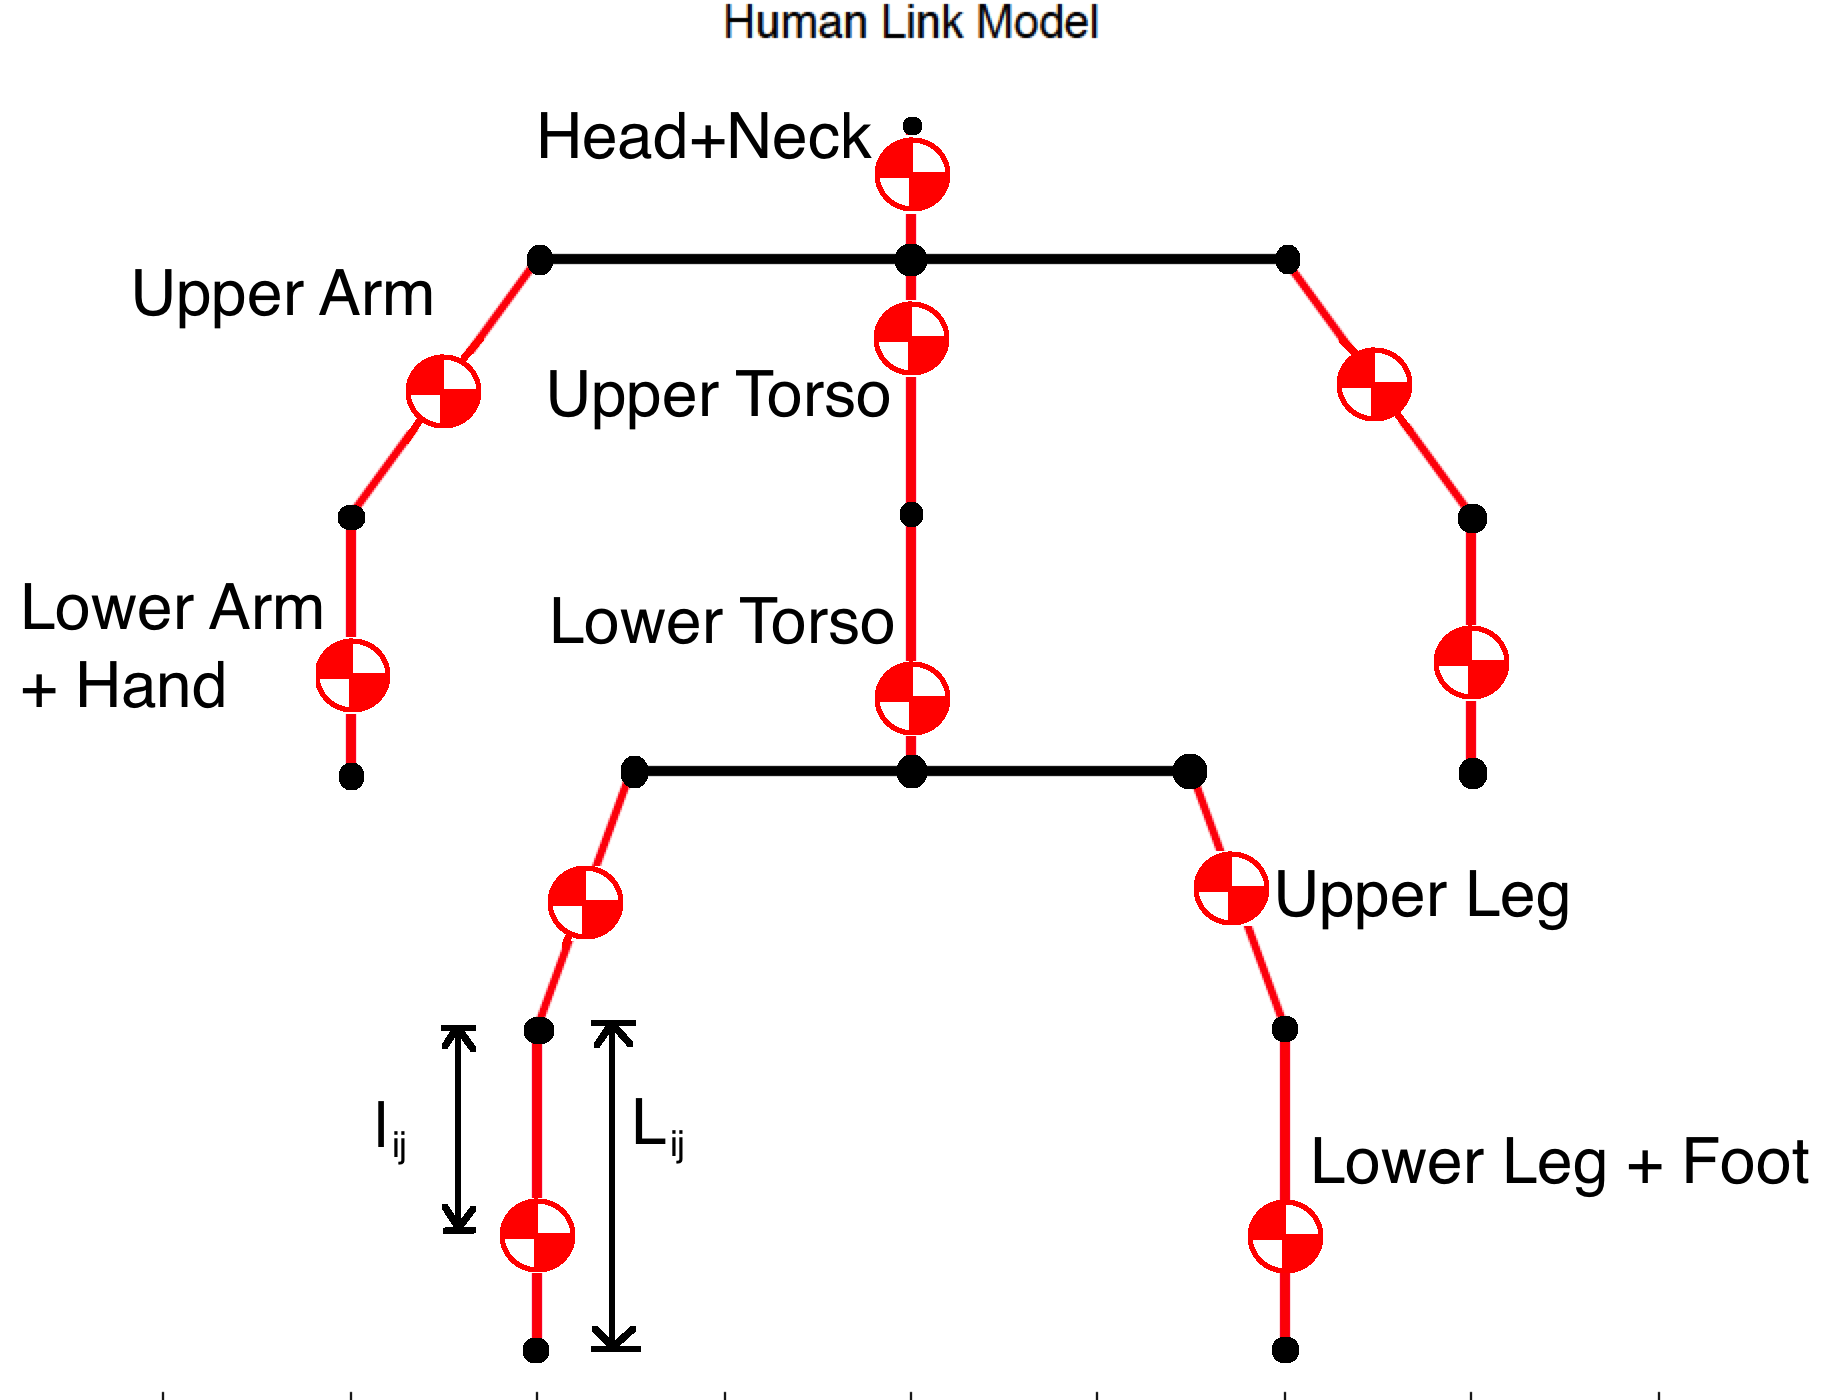
\includegraphics[width=0.9\columnwidth]{figures/skeleton3.png}
\caption{Chain approximation model of a human.}
\label{fig:humanmodel}
\end{figure}

Using this representation, the CoM  can be predicted as
\begin{equation}
\text{CoM} = \frac{1}{M}\sum_{(i,j)\in\mathcal{L}} m_{ij}(1-\rho_{ij})r_i + m_{ij}\rho_{ij}r_j
\end{equation}
where $M$ is the total mass of the human. Alternatively, 
\begin{equation}
\text{CoM} = \frac{1}{M}\sum_{(i,j)\in\mathcal{L}} m_{ij} r_i + m_{ij}\rho_{ij}(r_j - r_i) \label{eq:comSum}
\end{equation}
Consider a na\"ive method of solving for $m_{ij}$, $\rho_{ij}$ using least squares. In this case, we rewrite \eqref{eq:comSum} as, 
\begin{equation}
\text{CoM} = [r_1,  r_2 - r_1, \hdots r_i, r_j - r_i, \hdots] \theta \label{eq:comsingle}
\end{equation}
where
\begin{equation}
\theta = [\frac{m_{12}}{M}, \frac{m_{12}}{M}\rho_{12}, \hdots, \frac{m_{ij}}{M}, \frac{m_{ij}}{M}\rho_{ij}, \hdots]^T \nonumber
\end{equation}
%By estimating the parameter vector $\theta$ and observing the joint positions, one may predict the position of the center of mass as well as calculate the inertial parameters.
Then, given $K$ measurements, $k = 1,\hdots, K$, using superscript to denote measurement number, we concatenate \eqref{eq:comsingle} to receive
\begin{equation}
\begin{bmatrix}
\text{CoM}^1\\
\vdots \\
\text{CoM}^k \\
\vdots \\
\text{CoM}^K
\end{bmatrix}
= 
\begin{bmatrix}
r_1^1,  r_2^1 - r_1^1, \hdots r_i^1, r_j^1 - r_i^1, \hdots  \\
\vdots \\
r_1^k,  r_2^k - r_1^k, \hdots r_i^k, r_j^k - r_i^k, \hdots  \\
\vdots \\
r_1^K,  r_2^K - r_1^K, \hdots r_i^K, r_j^K - r_i^K, \hdots 
\end{bmatrix}
\theta
\label{eq:com}
\end{equation}
For convenience let $Q$ stand for the matrix in \eqref{eq:com}. In the case that a joint is shared by two or more links, i.e. $\exists i,j,k$ s.t. $\{(i,k),(k,j)\} \in \mathcal{L}$, as is the case in the human model, the matrix $Q$ has redundant columns and therefore is ill-conditioned. Regardless of the number of observations, one cannot solve for $\theta$ using least squares. 
This is due to an inherent observability problem when using only static observations. That is to say, when observing the center of mass during only static positions, it is impossible to delineate both how much a link weighs and where the center of mass lies along the link simultaneously. There exists a null space in which a change in the mass of a link coupled with a movement of the center of mass will result in identical center of mass observations. 
The formulations in \cite{gonzalez2012estimation, cotton2011estimation} use only static position measurements and therefore suffer from the same problem of observability. 


\section{BAYESIAN INFERENCE ALGORITHMS}
%\section{Bayesian Inference}
In order to account for the problem of observability mentioned in the previous section, we adopt a Bayesian probabilistic approach. 
Bayesian inference is a method for inferring the most probable parameters given the observations as well as prior distributional knowledge of the parameters. In this case, Bayesian 
inference fills in the missing information in the null space by supplementing the estimation process with prior distributional knowledge from the medical literature.
In this sense, Bayesian inference acts as a sort of regularization, which solves the problem of ill-posedness of $Q$. 
This section first reviews the fundamentals of Bayesian inference and then introduces the algorithms used for parameter estimation: MH and the PF.

% using a prior over link masses and center of masses obtained from the literature \cite{}.  The following section reviews Bayesian probability fundamentals as well as the algorithms used to determine $\theta$. 

\subsection{Bayesian Inference}
Bayesian inference is a method for determining the posterior probability distribution of a set of (unobservable) parameters given a set of observations as well as a prior distribution over the parameters. 
%In particular, it uses Baye's rule to update the probability density function (pdf) over a set of parameters using additional evidence that has been collected. 
More formally, consider a set of parameters of interest, $\theta$, a prior probability density function (pdf) over those parameters $p(\theta)$, a set of measurements $y$, and measurement likelihood pdf $p(y\mid \theta)$, parameterized by  $\theta$. Baye's rule states that the posterior distribution of the parameters $p(\theta \mid y)$ given the observations is
\begin{equation}
p(\theta \mid y) = \frac{1}{Z} p(y \mid \theta)p(\theta)
\end{equation}
where $Z = \int_\Theta p(y \mid \theta)p_\theta(\theta)$ and $\Theta = \{\theta \mid p(y \mid \theta)p_\theta(\theta)>0\}$. $Z$ is a normalization factor to ensure that $p(\theta \mid y)$ integrates to $1$ and is \emph{constant} for a fixed set of data. The value of $\theta$ with highest posterior probability, i.e. $\theta_{MAP} = \arg\max_\theta p(\theta \mid y)$, is called the the maximum a posteriori (MAP) estimate. In this work, after the MAP estimate has been approximately solved, the center of mass is calculated by plugging the MAP estimate into $\theta$ in \eqref{eq:comSum}.
%In applications where only the MAP estimate is considered, it is sufficient to drop the normalization constant and only consider the quantity $p(\theta \mid y) \propto p(y \mid \theta)p_\theta(\theta)$.

In general, it is impracticable or infeasible to calculate the normalization factor for all but special distributions. Therefore, a variety of approximation techniques must be used.
 %In this work, we consider three approximation methods. In the first method, we approximate the prior and measurement noise distributions as Gaussian. In this case, the posterior distribution can be calculated in closed form as another Gaussian. This approximation method has the benefit of being extremely fast in computation and algorithmic simplicity, however, it does not guarantee feasible assignments to parameters. That is to say, while in the original distribution, negative masses and center of masses are not permitted, a Gaussian distribution has infinite support, so it may return a MAP solution with negative values.
This paper considers two approximation methods, one batch and one online. The first approximation method, Metropolis Hasting (MH), is a member of the Markov Chain Monte Carlo (MCMC) framework \cite{chib1995understanding} and works for batch data. The MCMC algorithm generates samples from the posterior distribution $p(\theta \mid y)$, and one can then record the samples with the highest value of $p(\theta \mid y) \propto p(y \mid \theta)p(\theta)$ to approximately estimate the MAP solution. Since samples with high probability are drawn more frequently than those will low probability, MCMC generates good approximate MAP solutions in a relatively small number of samples. 

In general, MCMC works well for solving approximate MAP problems in which the dimensionality of the parameters is high or in which generating samples from the distribution is difficult due to a complicated distribution shape. In this work, the dimensionality of the parameters is quite large at $22$, 11 masses and 11 center of masses, and the prior distribution has many constraints.Therefore, MCMC is a natural fit for this estimation problem.
However, while a batch solution may work for many cases, one might also wish to have an online method for parameter estimation to permit some sort of active exploration of parameters. For example, \cite{ayusawa2009optimal,gonzalez2013online} provide feedback to the user during the training phase to move joints that have larger uncertainty.% given the current observations.

Thus, the second approximation method uses an online Particle Filter (PF) method \cite{doucet2009tutorial}. Using a PF, the probability distribution function is approximated using a set of weighted basis probability functions, or particles. After each new observation, the weight of each particle is adjusted according to the measurement likelihood function in order to reflect the new information. In this way, the posterior distribution can be approximated using a reduced basis set and simple multiplicative updates at each observation.

Both algorithms are first presented in their general form, and then the specific form of the likelihood and prior pdfs used in the experiments are presented in Section \ref{distribution}.

\subsection{Metropolis-Hasting}
MCMC is a set of algorithms in the statistics literature that are able to generate samples from a distribution for which direct sampling is difficult. In the work, we draw samples from the posterior distribution $p(\theta \mid y)$ and the specific algorithm used is the Metropolis-Hasting (MH) algorithm. The MH algorithm does not require the exact probability function $p(\theta \mid y)$ but simply a proportional function, in this case $p(y \mid \theta)p(\theta)$. 
The MH algorithm works by generating a random walk using some distribution which may be directly sampled, such as a uniform or Gaussian distribution, and then accepting or rejecting samples according to the relative likelihoods of the current sample and the proposed next sample.
For a more detailed explanation of the MH algorithm and its applications, see \cite{chib1995understanding}. 

The algorithm is initialized with an arbitrary parameter sample, $\theta_0$. In this work, $\theta_0$ is drawn from the prior distribution, $\theta_0 \sim p(\theta)$. Then, at every iteration, the MH algorithm proposes a new sample by perturbing the current sample $\theta' \sim f(\theta_{i})$ according to some distribution that is simple to sample. 
In this work, at every iteration, the algorithm adds white Gaussian noise to the current sample $\theta' \sim \mathcal{N}(\theta{t},\sigma_{MH}^2)$. With some probability, the new sample is then accepted or rejected using the relative posterior probabilities of the samples, i.e. with probability $\alpha = \min\left(1, \frac{p(\theta' \mid y)}{p(\theta_{t} \mid y)}\right)$ the new sample is accepted and $\theta_{t+1} = \theta'$, or the sample is rejected so $\theta_{t+1} = \theta_t$. By accepting proposed samples with this modified probability, it can be shown that the resulting distribution, as the number of samples drawn tends to infinity, is the true posterior distribution \cite{chib1995understanding}.
This work focuses on estimating the MAP solution, so in addition, the sample with the highest posterior probability is saved.

Lastly, while in theory the MH algorithm will return samples from the target distribution as the number of iterations tends to infinity, in practice %there is a burn-in period in which the initial state $\theta_0$ creates a bias of samples, and a 
the MH may become stuck in local optima. Therefore, random restarts are needed to ensure proper mixing and prevent convergence to local optima. Determining when to perform random restarts is somewhat domain and user dependent, however, in this work, we perform a restart when the sample hasn't changed for over $1000$ iterations.
The algorithm is formalized in Algorithm \ref{alg:mh}.

\begin{algorithm}
\begin{algorithmic}[1]
\caption{Approximate MAP via Metropolis Hasting}
\label{alg:mh}
\STATE \textbf{Input:} Prior distribution $p(\theta)$, likelihood function $p(y \mid \theta)$, random walk distribution $\mathcal{N}(0,\sigma_{MH}^2)$
\STATE Initialize sample $\theta_0 \sim p(\theta)$, $\hat \theta_{MAP} = \theta_0$
\WHILE{Samples are needed}
\STATE Generate new candidate $\theta' = \theta_{t} + \nu$, $\nu \sim \mathcal{N}(0,\sigma_{MH}^2)$
\STATE Calculate acceptance probability $\alpha = \min\left(1,\frac{p(y \mid \theta' )p(\theta')}{p(y \mid \theta_t )p(\theta_t)}\right)$
\STATE Generate $b \sim \text{Uniform}(0,1)$.
\IF{$b <\alpha$}
\STATE Accept new sample, $\theta_{t+1} = \theta'$.
\ELSE
\STATE Reject new sample, $\theta_{t+1} = \theta_t$.
\ENDIF
\IF{$p(y \mid \theta_{t+1} )p(\theta_{t+1}) > p(y \mid \hat \theta_{MAP} )p(\hat \theta_{MAP})$}
\STATE $\hat \theta_{MAP} = \theta_{t+1}$
\ENDIF
\IF{$\theta_t$ remains unchanged for $1000$ iterations}
\STATE Random restart: $\theta_{t+1} \sim p(\theta)$ 
\ENDIF
\ENDWHILE
\end{algorithmic}
\end{algorithm}

\subsection{Particle Filter}
While the MH algorithm works well for finding the approximate MAP solution, it is constrained to batch data. In order to generate a MAP solution or give feedback during training, the particle filter (PF) is used as an online method for finding the approximate MAP solution.
For a detailed introduction to the PF, refer to \cite{doucet2009tutorial}.

The PF approximates the posterior distribution using a set of basis functions, such as the Dirac delta function or a Gaussian distribution with narrow bandwidth. In this work, the posterior distribution is approximated using Dirac delta functions as 
\begin{equation}
\hat p(\theta \mid y) = \sum_i w_i \delta(\theta - \theta_i)
\end{equation}
where $\delta(\theta - \theta_i)$ is the dirac delta, which is zero everywhere except for $\delta(0) = \infty$, and integrates to one, $\int_\Theta \delta =1$. In order to ensure that $\hat p (\theta \mid y)$ is a valid probability distribution, i.e. integrates to one and is nonnegative, the weights have the properties $\sum_i w_i  =1$ and $\forall i,$ $w_i \geq 0$.

The PF is initialized by drawing particles $\theta_i \sim p(\theta)$ from the prior distribution. The weights are initialized to $w'_i = p(\theta_i)$ and then normalized as $w_i = w'_i / \sum_i w'_i$. 
Given a new observation $y^t$, the weights of the particles must be updated to reflect the modified posterior distribution. In particular, one may write the updated posterior probability as
\begin{equation}
 p(\theta \mid y^1, \hdots, y^t) \propto p(y^1, \hdots,y^t \mid \theta)p(\theta) \label{eq:condind1}
\end{equation}
and it follows that due to the conditional indendence of the observations conditioned on the parameters $\theta$, \eqref{eq:condind1} can be rewritten as,
\begin{equation}
 p(\theta \mid y^1, \hdots, y^t) \propto \prod_{i=1}^t p(y^i\mid \theta)p(\theta) \label{eq:condind2}
\end{equation}
Or written recursively as,
\begin{equation}
 p(\theta \mid y^1, \hdots, y^t) \propto p(\theta \mid y^1, \hdots, y^{t-1})p(y^t\mid \theta) \label{eq:condind3}
\end{equation}

Therefore, the weights are updated as $w_i^t = w_i^{t-1}p(y^t \mid \theta)$ and then again normalized. Finding the MAP solution at iteration $t$ requires only searching over the weights $w_i$ and returning the corresponding $\hat \theta_{MAP} = \theta_{j}$, where $j = \arg\max_i w_i$.

In practice, after many observations, many of the weights become negligibly close to zero, as the posterior probability $p(\theta_i \mid y^1,\hdots,y^t)$ goes to zero. Therefore, in order to maintain coverage over the regions with high probability, particles are deleted and resampled close to particles with higher weight. Many techniques exist for resampling, however, our approach is detailed in Algorithm \ref{alg:pf}, line \ref{line:res}. Essentially, every iteration, the algorithm deletes 10\% of the particles with the lowest weight and resamples. For resampling, the algorithm choses an existing particle $\theta_j$ with probability proportional to the weight of the particle $w_j$ or choses to generate a new particle from the prior $\theta_k \sim p(\theta)$ with probability $\alpha_{PF}$. If an existing particle is chosen, a new particle $\theta_k \sim \mathcal{N}(\theta_j,\sigma_{PF}^2)$ is created close to the old particle. 
The weight is initialized as $w'_k = p(\theta)p(y_1,\hdots,y_t \mid \theta)$.
This process is formalized in Algorithm \ref{alg:pf}. 

\begin{algorithm}
\begin{algorithmic}[1]
\caption{Approximate MAP via Particle Filter}
\label{alg:pf}
\STATE \textbf{Input:} Prior distribution $p(\theta)$, likelihood function $p(y \mid \theta)$, particle generation distribution $\mathcal{N}(0,\sigma_{PF}^2)$, number of particles $K$
\STATE Initialize particles $k = 1,\hdots,K$, $\theta_k \sim p(\theta)$.
\STATE Calculate probability $w'_k = p(\theta)$
\STATE Calculate normalized weights $w_k = \frac{w'_k}{\sum_i w'_k}$
\STATE Calculate approximate MAP $j = \arg\max_i w_i$, $\hat \theta_{MAP} = \theta_j$
\WHILE{Observations are available}
	\STATE Observe new datapoint $y_t$
	\STATE Update probabilities $\forall k, w'_k = w'_k p(y_t \mid \theta_k)$.
	\STATE Calculate normalized weights $\forall k$, $w_k = \frac{w'_k}{\sum_i w'_k}$.
	\STATE Estimate MAP $j = \arg\max_i w_i$; $\hat \theta_{MAP} = \theta_j$
	\FOR{Each particle $\theta_k$ with weight in the lowest 10\% percentile}
		
			\STATE Delete particle $\theta_k$
			\STATE Sample from multinomial distribution $\text{Multi}(w_1,\hdots, w_K, \alpha_{PF})$ \label{line:res}
			\IF{Particle $\theta_j$ selected}
				\STATE Sample $\theta_k \sim \mathcal{N}(\theta_j, \sigma^2_{PF})$
			\ELSE
				\STATE Sample $\theta_k \sim p(\theta)$
			\ENDIF
			\STATE Set $w'_k = p(\theta)p(y_1,\hdots,y_t \mid \theta)$ 
	\ENDFOR
\ENDWHILE
\end{algorithmic}
\end{algorithm}











\section{EXPERIMENTS AND RESULTS}
This section describes the distributions used in the MH and PF algorithms as well as experiments used for validation.

\subsection{Distributions and Parameters}
\label{distribution}
In order to use Bayesian algorithms, one must designate a prior which generally captures the structure of the true prior distribution. As more data becomes available, the prior has less effect on the MAP solution, so for data rich applications, the exact formulation of the prior is not as important. Since the weight and dimensions of each human operator will be different, we non-dimensionalize the distribution by considering the distribution over mass fraction (i.e. $\frac{m_{ij}}{\sum m_{ij}}$) and the distance of the center of mass relative to the link length, $\rho_{ij}$. 

In the experiments section, the prior over the masses and center of masses is modeled as a Gaussian with truncated tails and hard constraints that the body masses are symmetric and that the mass sums to one. 
The mean and standard deviation over the masses $m_{ij}$ and center of masses $\rho_{ij}$ are derived primarily from \cite{jensen1989changes,armstrong1988anthropometry} and are listed in Table \ref{table:prior}. 
The tails are truncated such that no body part has negative mass and such that the center of mass is contained within the link modeling the body part.
Additionally, we constrain the distribution such that left-right symmetry is maintained and such that the masses sum to one. Mathematically,
\begin{equation}
p(\theta) \propto
\left\{
  \begin{array}{lc}
    	0& : \sum m_{ij} \neq 1 \\
	0& : \exists m_{ij} < 0 \\
	0& : \exists \rho_{ij} < 0 \\
	0& : \exists \rho_{ij} > 1 \\
	0& : \text{Not symmetric}  \\
    	\mathcal{N}(\mu_\theta,\Sigma_\theta) & : \text{otherwise}
    
  \end{array}
\right.
\end{equation}
where the mean values and variances are given in Table \ref{table:prior}.
The measurement likelihood function is modeled as a Gaussian with mean given by the right hand side of \eqref{eq:comSum}, with variance $\omega^2 = 100^2\text{mm}^2$,
\begin{equation}
p(y \mid \theta, r) = \mathcal{N}(\sum_{(i,j)\in\mathcal{L}} m_{ij} r_i + m_{ij}\rho_{ij}(r_j - r_i), 100^2)
\end{equation}

\begin{table}
\caption{Parameters for Prior Distribution}
\label{table:prior}
\begin{center}
\begin{tabular}{|c|c|c|}
\hline
           & m (mean, variance) & $\rho$ (mean, variance) \\
\hline
 Head+Neck & $(0.0775, 0.05^2)$ & $(0.5344, 0.05^2)$ \\
\hline
 Upper Torso & $(0.1284, 0.05^2)$ & $(0.5529, 0.05^2) $\\
\hline
 Lower Torso & $(0.7233, 0.05^2)$ & $(0.4903, 0.05^2) $\\
\hline
 Upper Arm & $(0.0401, 0.05^2)$ & $(0.5503, 0.05^2)$ \\
\hline
 Lower Arm+Hand & $(0.0291, 0.05^2)$ & $(0.7115, 0.05^2)$ \\
\hline
 Upper Leg & $(0.0987, 0.05^2)$ & $(0.4482, 0.05^2) $\\
\hline
 Lower Leg+Foot & $(0.0364, 0.05^2)$ & $(0.5797, 0.05^2)$ \\
\hline
\end{tabular}
\end{center}
\end{table}

%\begin{table*}
%\caption{Parameters for Prior Distribution}
%\label{table:prior}
%\begin{center}
%\begin{tabular}{|c|c|c|c|c|c|c|c|}
%\hline
% &Head+Neck & Upper Torso & Lower Torso & Upper Arm & Lower Arm+Hand & Upper Leg & Lower Leg+Foot\\
%\hline
% $m$ Fraction Mean &0.0775 & 0.1284 & 0.2733 & 0.0401 & 0.0291 & 0.0987& 0.0364 \\
%\hline
% $m$ Fraction Variance & $0.05^2$ & $0.05^2$ & $0.05^2$ & $0.05^2$ & $0.05^2$ & $0.05^2$ & $0.05^2$\\
%\hline
% $\rho$ Mean &0.5433& 0.5529 & 0.4903 & 0.5503 & 0.7115 & 0.4482 & 0.5797 \\
%\hline
% $\rho$ Variance & $0.05^2$ & $0.05^2$ & $0.05^2$ & $0.05^2$ & $0.05^2$ & $0.05^2$ & $0.05^2$\\
%\hline
%\end{tabular}
%\end{center}
%\end{table*}
%\begin{tabularx}{\textwidth}
%\caption{Parameters for Prior Distristribution}
%\label{table:prior}
 % \toprule
%  xx&1&2&3\\
%  xx&1&2&3\\
%  \bottomrule
%\end{tabularx}

In the experiments, the following parameters were used for the MH and PF algorithms: $\sigma_{PF} = 0.005$, $\alpha_{PF} = 0.01$, $K=100$, and $\sigma_{MH} = 0.01$.

\subsection{Experiments}
\label{experiments}
In order to validate the methods for parameter identification and center of mass prediction, five subjects were tested. 
Each subject performed in two trials. In each trial, the subject moved slowly and demonstrated a variety of different poses for approximately two minutes. 
The first of these trials was used as a training dataset by the algorithms to estimate the mass distribution, and the second data trial was used as a validation, or test, dataset. 
In addition to testing the MH and PF algorithms, we also compare our methods to the SECS model of \cite{gonzalez2012estimation}, which does not estimate the mass distribution but estimates regression coefficients that can be used to predict the center of mass from angle positions.

We compare the predicted center of mass to that measured by the Wii balance board on the second \emph{testing dataset}, which is different from the first dataset used to train the algorithms. For testing CoM prediction, the MH and PF MAP estimates are plugged into $\theta$ of \eqref{eq:comSum}. 
There is no way to directly measure the inertial parameters of the human, so this paper simply compares the output of these algorithms to the prior distribution. Further work will focus on other validation methods.

A Kinect camera estimates the pose of the human using the built-in skeleton detection algorithm, with sampling frequency approximately 30~Hz. The wii balance board records the center of pressure, which is assumed to be close to the center of mass, in the horizontal place at approximately 60~Hz. 
Both Kinect and balance board measurements are first filtered using a median filter and then a sliding average filter. The median filter considers the nearest 7 measurements and is used to filter outliers that sporadically occur when the Kinect skeleton detection algorithm loses track of the skeleton. The sliding window filter has the purpose of both filtering noise as well as accounting for different sensor sampling rates. In particular, the sliding average filter interpolates the observation value by taking a weighted moving average of all observations within a $0.1$~s window. %using a window shape $\frac{1}{1+\beta(\Delta T)^2}$.
%: $\hat y = \sum \frac{1}{1+(\Delta T)^2} y_i$


Table \ref{table:RMSE} compares the mean absolute error (MAE) predicting the center of mass for each person. Figure \ref{fig:com1} shows example CoM trajectories and predictions for the test trials. Lastly, table \ref{table:massdist} shows the inertial parameter estimates compared with the initial prior estimates for one subject.
\begin{table}
\caption{CoM Prediction MAE (mm)}
\label{table:RMSE}
\begin{center}
\begin{tabular}{|c|c|c|c|c|c|}
\hline
 & Subject 1 & Subject 2 & Subject 3 & Subject 4 & Subject 5\\
\hline
MH & 28.87   & 27.88 & 30.59 & 16.56 & 22.13\\
\hline
PF & 27.68 1 & 27.43 & 30.69 & 18.79 & 23.44\\
\hline
SESC & 60.06 & 65.92 & 43.49 & 42.52 &  59.9\\
\hline
\end{tabular}
\end{center}
\end{table}








\begin{table*}[t]
\caption{Mass Distribution for Subject 1-5. Parameters listed in tuples ($m$ fraction, $\rho$)}
\label{table:massdist}
\begin{center}
\begin{tabular}{|c|c|c|c|c|c|c|c|}
\hline
 &Head+Neck & Upper Torso & Lower Torso & Upper Arm & Lower Arm+Hand & Upper Leg & Lower Leg+Foot\\
\hline
\hline
 Prior Mean &(0.0775,0.5433) & (0.1284,0.5529) & (0.2733,0.4903) & (0.0401,0.5503) & (0.0291,0.7115) & (0.0987,0.4482) & (0.0364,0.5797) \\
\hline
  \multicolumn{8}{|c|}{Subject 1} \\
\hline
 MH Estimate &(0.0494,0.5408) & (0.1193,0.5216) & (0.4394,0.5523) & (0.0149,0.5704) & (0.0107,0.7185) & (0.0891,0.3708) & (0.0812,0.6379) \\
\hline
 PF Estimate & (0.0349,0.5473) & (0.1436,0.5288) & (0.4051,0.5231) & (0.0218,0.5505) & (0.0095,0.7140) &  (0.1050,0.4064) & (0.0720,0.6088) \\
\hline
  \multicolumn{8}{|c|}{Subject 2} \\
\hline
 MH Estimate & (0.0140,0.5119) & (0.1142,0.5441) & (0.3929,0.5773) & (0.1077,0.5245) & (0.0099,0.7074) & (0.1120,0.4275) & (0.0099,0.6768) \\
\hline
 PF Estimate & (0.0105,0.5382) & (0.1446,0.5503) & (0.3340,0.5151) & (0.1015,0.5759) & (0.0098,0.7066) & (0.1003,0.4364) & (0.0439,0.6333) \\
\hline
  \multicolumn{8}{|c|}{Subject 3} \\
\hline
 MH Estimate & (0.0134,0.4719) & (0.3422,0.4982) & (0.3965,0.4678) & (0.0104,0.5116) & (0.0104,0.6882) & (0.0240,0.4320) & (0.0791,0.6881) \\
\hline
 PF Estimate & (0.0447,0.5175) & (0.2877,0.5700) & (0.3630,0.4720) & (0.0097,0.5552) & (0.0098,0.7222) & (0.0713,0.4346) & (0.0616,0.6032) \\
\hline
  \multicolumn{8}{|c|}{Subject 4} \\
\hline
 MH Estimate & (0.0134,0.4697) & (0.3422,0.5451) & (0.3965,0.6114) & (0.0102,0.5240) & (0.0102,0.6835) & (0.0460,0.4088) & (0.0843,0.6842) \\
\hline
 PF Estimate & (0.1046,0.5346) & (0.1953,0.5393) & (0.3384,0.4792) & (0.0103,0.5522) & (0.0101,0.7028) & (0.0876,0.4313) & (0.0729,0.5962) \\
\hline
  \multicolumn{8}{|c|}{Subject 5} \\
\hline
 MH Estimate & (0.1943,0.5992) & (0.0255,0.4678) & (0.4212,0.5487) & (0.0106,0.5193) & (0.0106,0.6784) & (0.0360,0.4140) & (0.1223,0.6899) \\
\hline
 PF Estimate & (0.1219,0.5746) & (0.1332,0.5386) & (0.3436,0.5075) & (0.0098,0.5506) & (0.0173,0.7232) & (0.0581,0.4261) & (0.1154,0.6448) \\
\hline
\end{tabular}
\end{center}
\end{table*}














%\begin{table*}[h]
%\caption{Mass Distristribution for Subject 1-5}
%\label{table:massdist}
%\begin{center}
%\begin{tabular}{|c|c|c|c|c|c|c|c|}
%\hline
% &Head+Neck & Upper Torso & Lower Torso & Upper Arm & Lower Arm+Hand & Upper Leg & Lower Leg+Foot\\
%\hline
% $m$ Fraction Prior Mean &0.0775 & 0.1284 & 0.2733 & 0.0401 & 0.0291 & 0.0987& 0.0364 \\
%\hline
% $\rho$ Prior Mean &0.5433& 0.5529 & 0.4903 & 0.5503 & 0.7115 & 0.4482 & 0.5797 \\
%\hline
%\hline
% Subject 1& & & & & &  & \\
%\hline
% $m$ Fraction MH Estimate &0.0494 & 0.1193 & 0.4394 & 0.0149 & 0.0107 & 0.0891& 0.0812 \\
%\hline
% $m$ Fraction PF Estimate & 0.0349 & 0.1436 & 0.4051 & 0.0218 & 0.0095 &  0.1050 & 0.0720 \\
%\hline
%
% $\rho$ MH Estimate &0.5408& 0.5216 & 0.5523 & 0.5704 & 0.7185 & 0.3708 & 0.6379 \\
%\hline
% $\rho$ PF Estimate &0.5473 & 0.5288 & 0.5231 & 0.5505 & 0.7140 & 0.4064 & 0.6088 \\
%
%
%\hline
%\hline
% Subject 2& & & & & &  & \\
%\hline
% $m$ Fraction MH Estimate &0.0140 & 0.1142  & 0.3929 & 0.1077 & 0.0099 & 0.1120 & 0.0099 \\
%\hline
% $m$ Fraction PF Estimate & 0.0105 & 0.1446 & 0.3340 & 0.1015 & 0.0098 &  0.1003 & 0.0439 \\
%\hline
% $\rho$ MH Estimate &0.5119& 0.5441 & 0.5773 & 0.5245 & 0.7074 & 0.4375 & 0.6768 \\
%\hline
% $\rho$ PF Estimate &0.5382 & 0.5503 & 0.5151 & 0.5759 & 0.7066 & 0.4364 & 0.6333 \\ 
%
%\hline
%\hline
% Subject 3& & & & & &  & \\
%\hline
% $m$ Fraction MH Estimate &0.0134 & 0.3422  & 0.3965 & 0.0104 & 0.0104 & 0.0240 & 0.0791 \\
%\hline
% $m$ Fraction PF Estimate & 0.0447 & 0.2877 & 0.3630 & 0.0097 & 0.0098 &  0.0713 & 0.0616 \\
%\hline
% $\rho$ MH Estimate &0.4719& 0.4982 & 0.4678 & 0.5116 & 0.6882 & 0.4320 & 0.6881 \\
%\hline
% $\rho$ PF Estimate &0.5175 & 0.5700 & 0.4720 & 0.5552 & 0.7222 & 0.4346 & 0.6032 \\
%
%\hline
%\hline
% Subject 4& & & & & &  & \\
%\hline
% &Head+Neck & Upper Torso & Lower Torso & Upper Arm & Lower Arm+Hand & Upper Leg & Lower Leg+Foot\\
%\hline
% $m$ Fraction MH Estimate &0.0134 & 0.3422  & 0.3965 & 0.0102 & 0.0102 & 0.0460 & 0.0843 \\
%\hline
% $m$ Fraction PF Estimate & 0.1046 & 0.1953 & 0.3384 & 0.0103 & 0.0101 &  0.0876 & 0.0729 \\
%\hline
% $\rho$ MH Estimate &0.4697& 0.5451 & 0.6114 & 0.5240 & 0.6835 & 0.4088 & 0.6842 \\
%\hline
% $\rho$ PF Estimate &0.5346 & 0.5393 & 0.4792 & 0.5522 & 0.7028 & 0.4313 & 0.5962 \\
%
%\hline
%\hline
% Subject 5& & & & & &  & \\
%\hline
% &Head+Neck & Upper Torso & Lower Torso & Upper Arm & Lower Arm+Hand & Upper Leg & Lower Leg+Foot\\
%\hline
% $m$ Fraction MH Estimate &0.1943 & 0.0255  & 0.4212 & 0.0106 & 0.0106 & 0.0360 & 0.1223 \\
%\hline
% $m$ Fraction PF Estimate & 0.1219 & 0.1332 & 0.3436 & 0.0098 & 0.0173 &  0.0581 & 0.1154 \\
%\hline
% $\rho$ MH Estimate &0.5992& 0.4678 & 0.5487 & 0.5193 & 0.6784 & 0.4140 & 0.6899 \\
%\hline
% $\rho$ PF Estimate &0.5746 & 0.5386 & 0.5075 & 0.5506 & 0.7232 & 0.4261 & 0.6448 \\
%\hline
%\end{tabular}
%\end{center}
%\end{table*}

\begin{figure}
\centering
\vskip -2cm
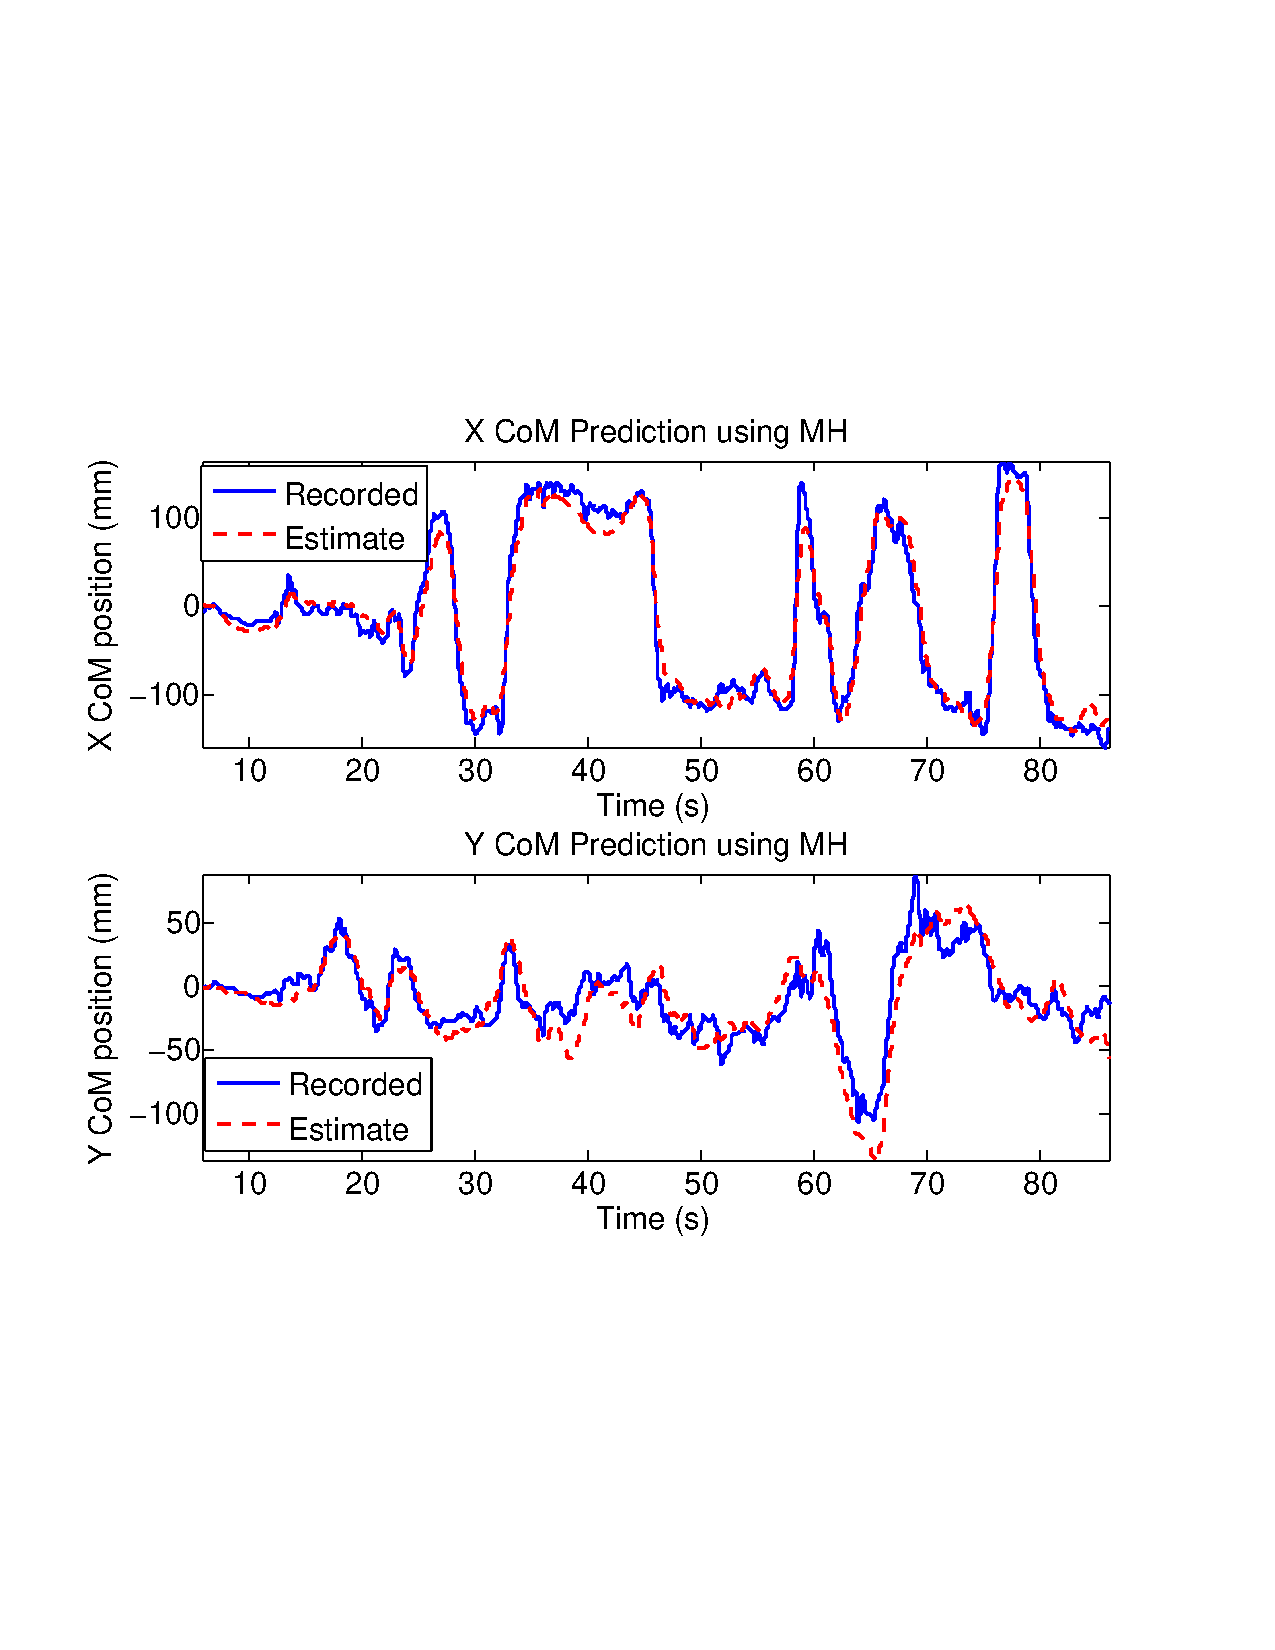
\includegraphics[trim=1cm 6cm 2cm 4cm, clip=true, width=\columnwidth]{figures/MH_Test2.pdf} 
\vskip -0.5cm
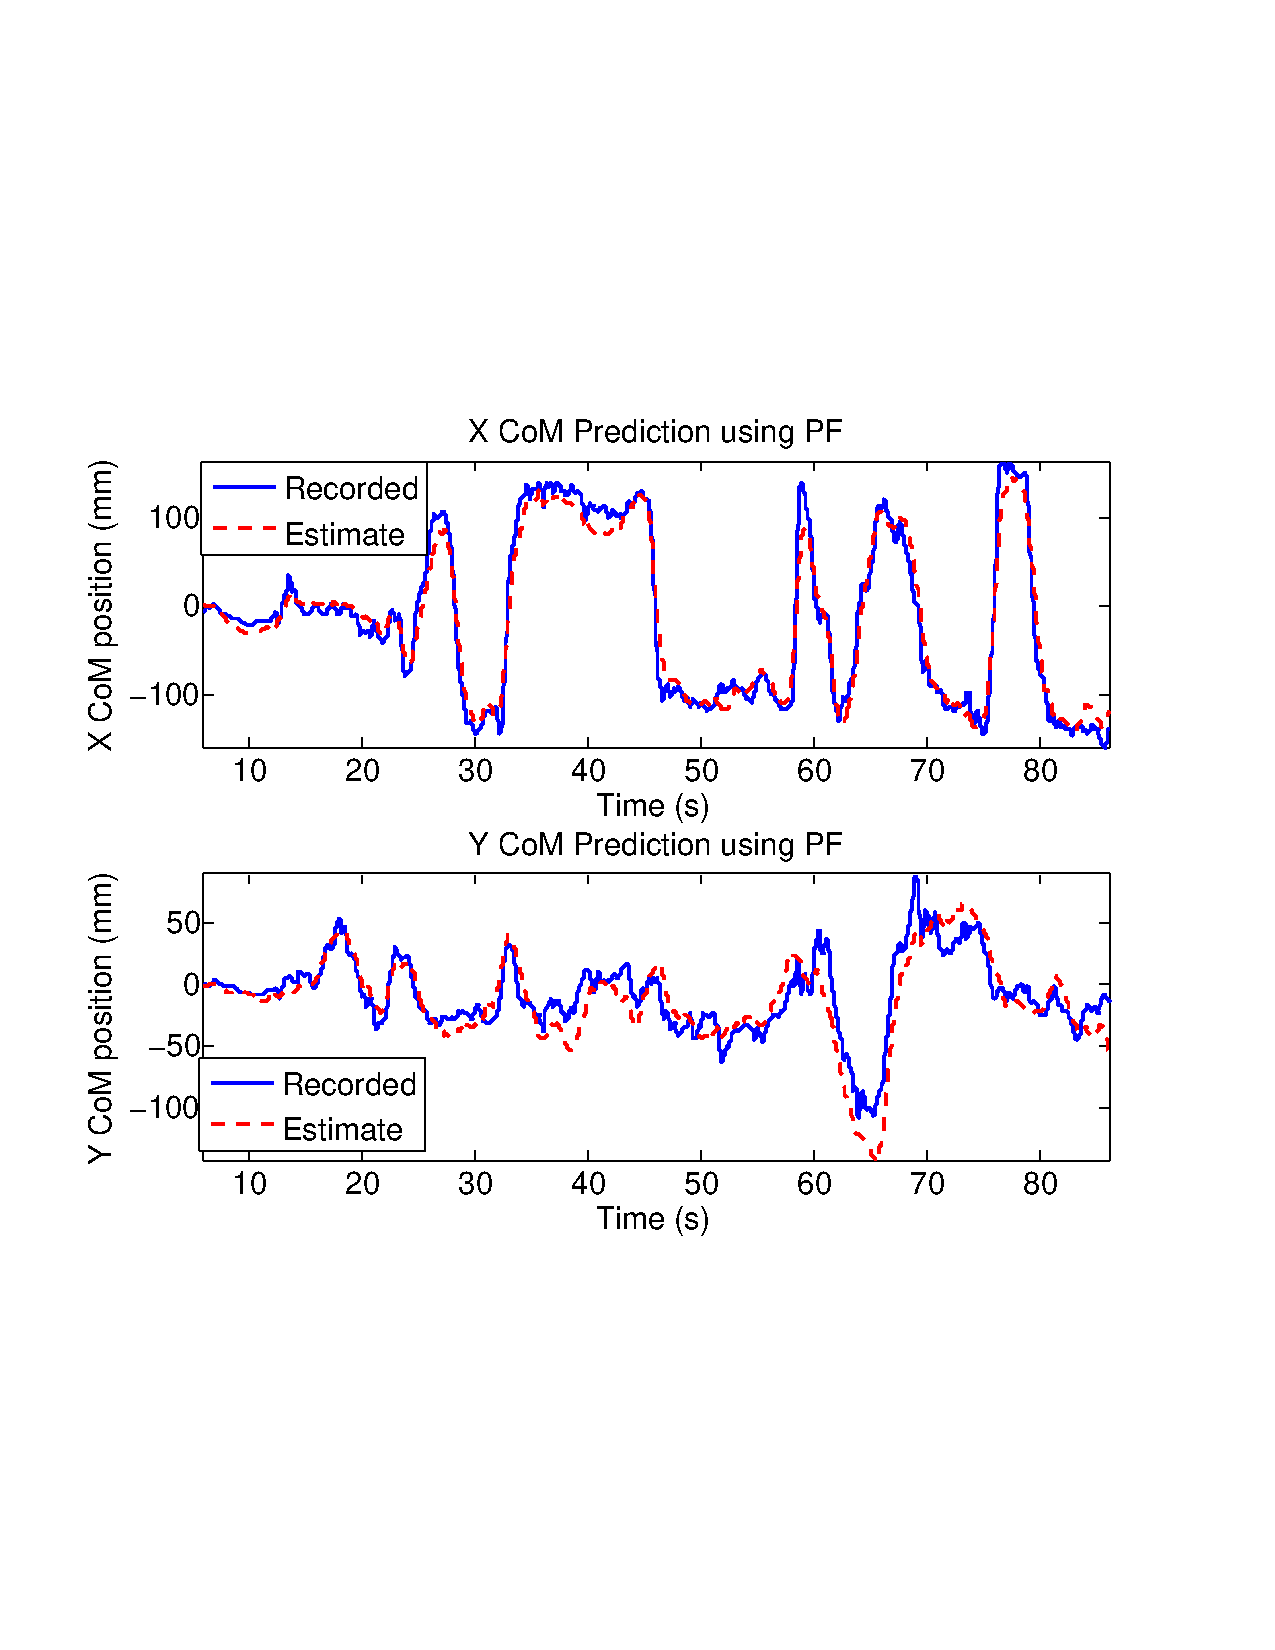
\includegraphics[trim=1cm 6cm 2cm 4cm, clip=true, width=\columnwidth]{figures/PF_Test2.pdf}
\vskip -0.5cm
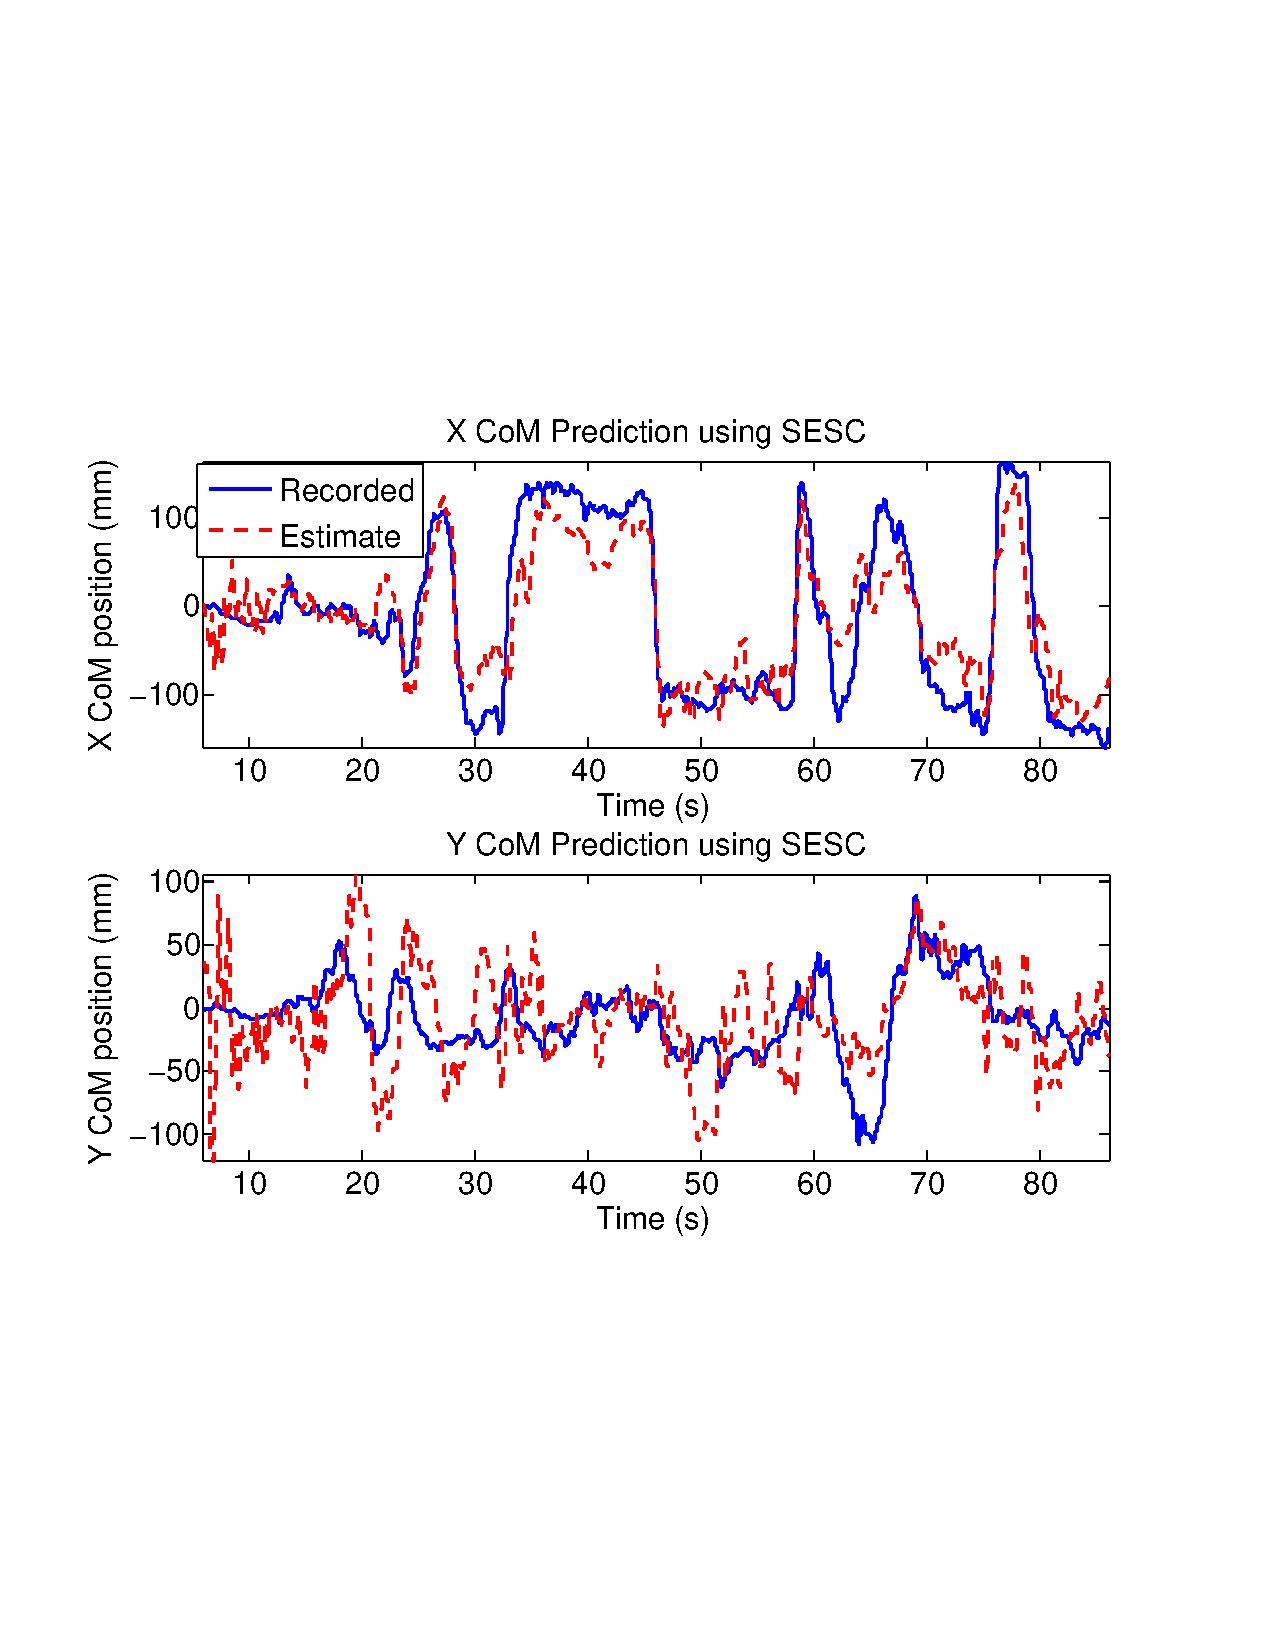
\includegraphics[trim=1cm 6cm 2cm 4cm, clip=true, width=\columnwidth]{figures/SESC_Test2.pdf}  
%   
\caption{CoM prediction using (Top) MH, (Middle) PF, (Bottom) SESC}
\label{fig:com1}
\end{figure}

%\begin{figure*}
%\begin{tabular}{ccc}
%\begin{subfigure}
%  \centering
%    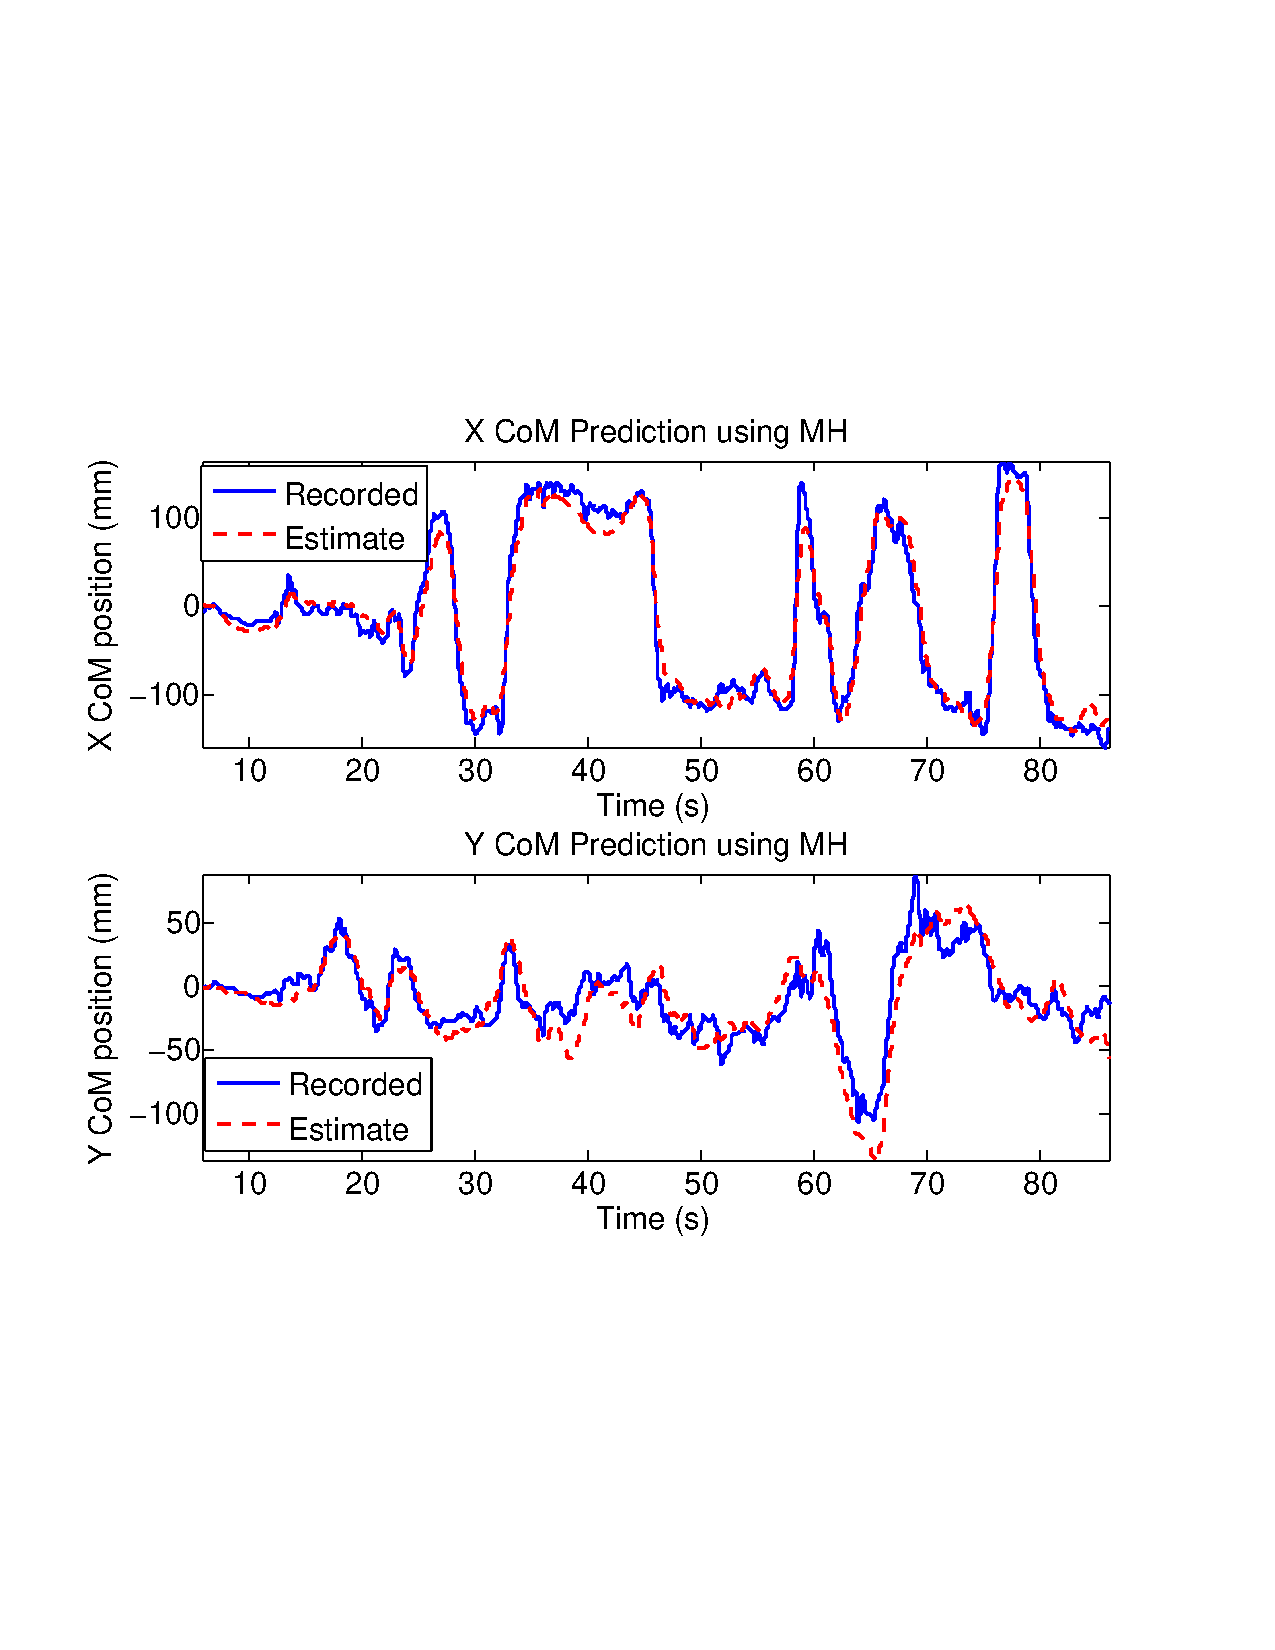
\includegraphics[trim=1cm 6cm 2cm 4cm, clip=true, width=0.6\columnwidth]{figures/MH_Test2.pdf} 
%\end{subfigure} &
%\hspace{-0.3in}
%\begin{subfigure}
%  \centering
%    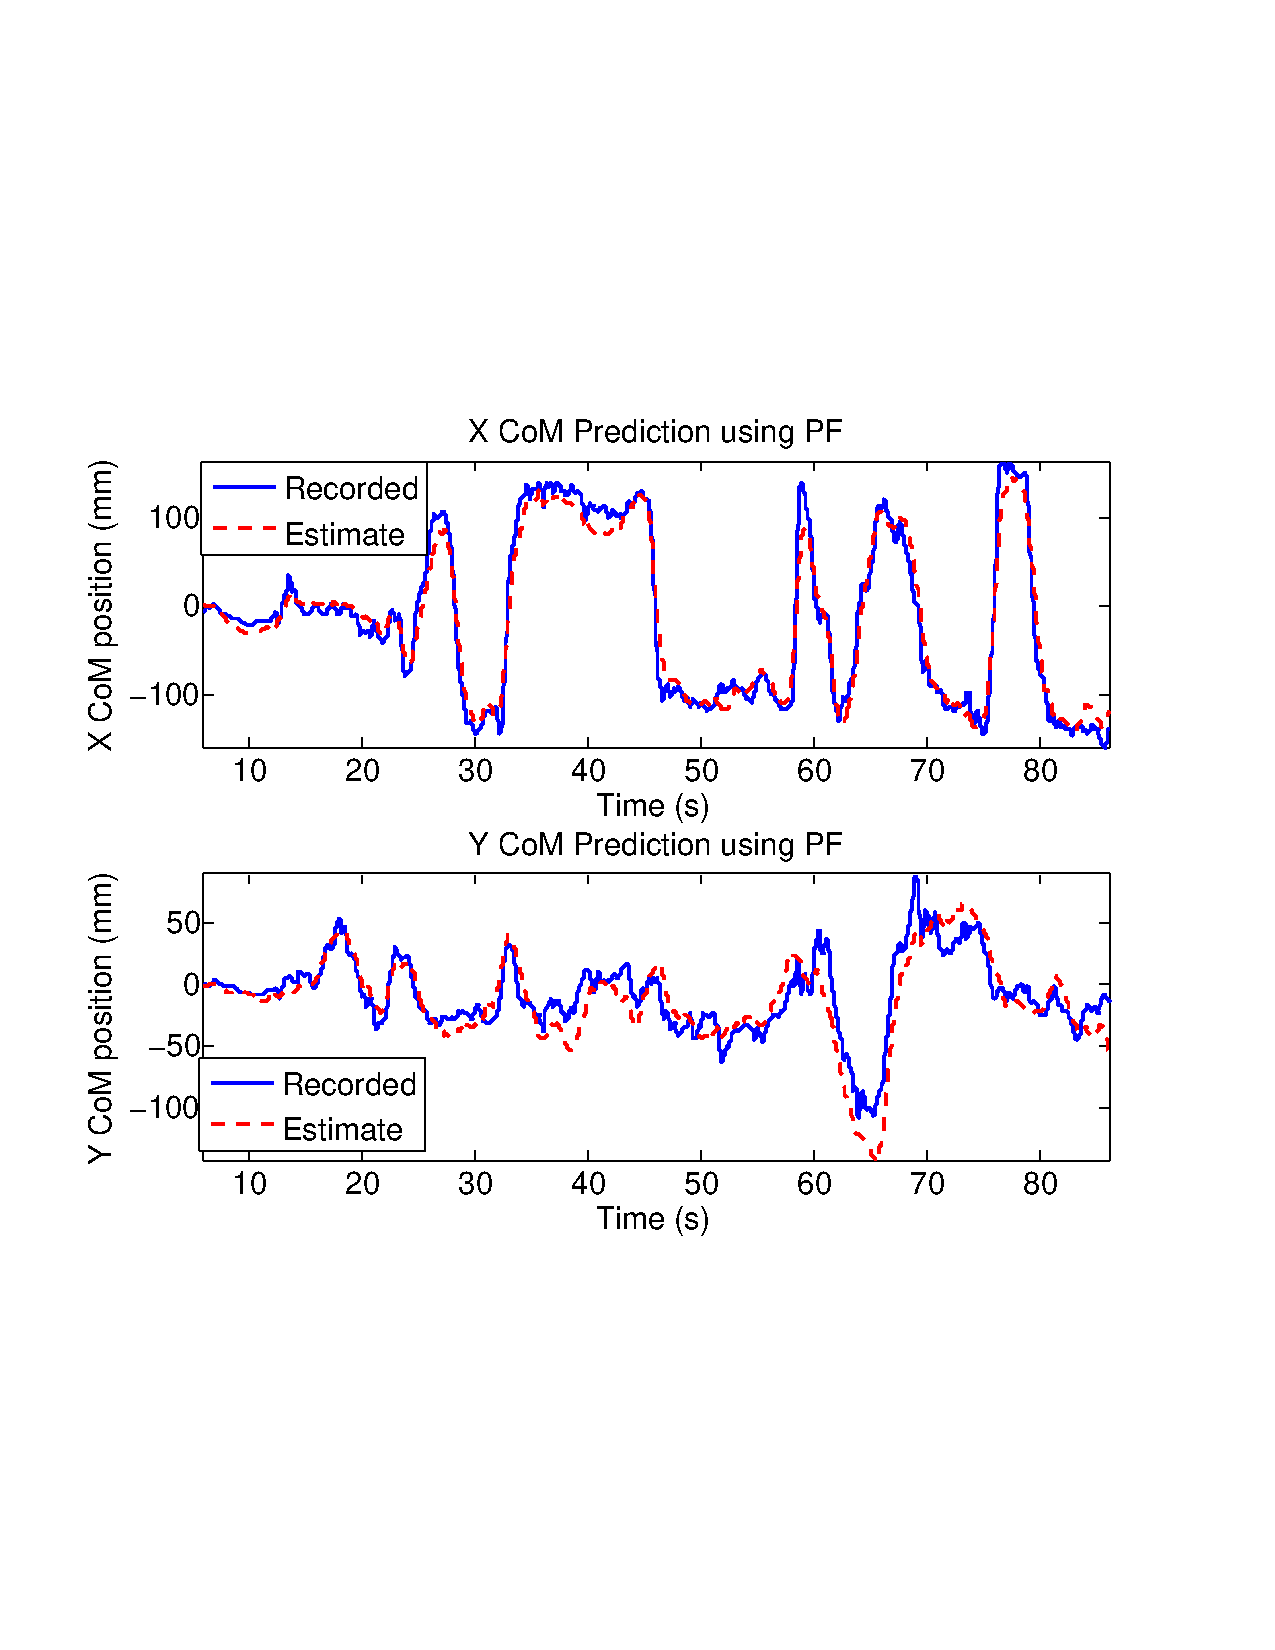
\includegraphics[trim=1cm 6cm 2cm 4cm, clip=true, width=0.6\columnwidth]{figures/PF_Test2.pdf} 
%\end{subfigure} &
%\hspace{-0.3in}
%\begin{subfigure}
%  \centering
%    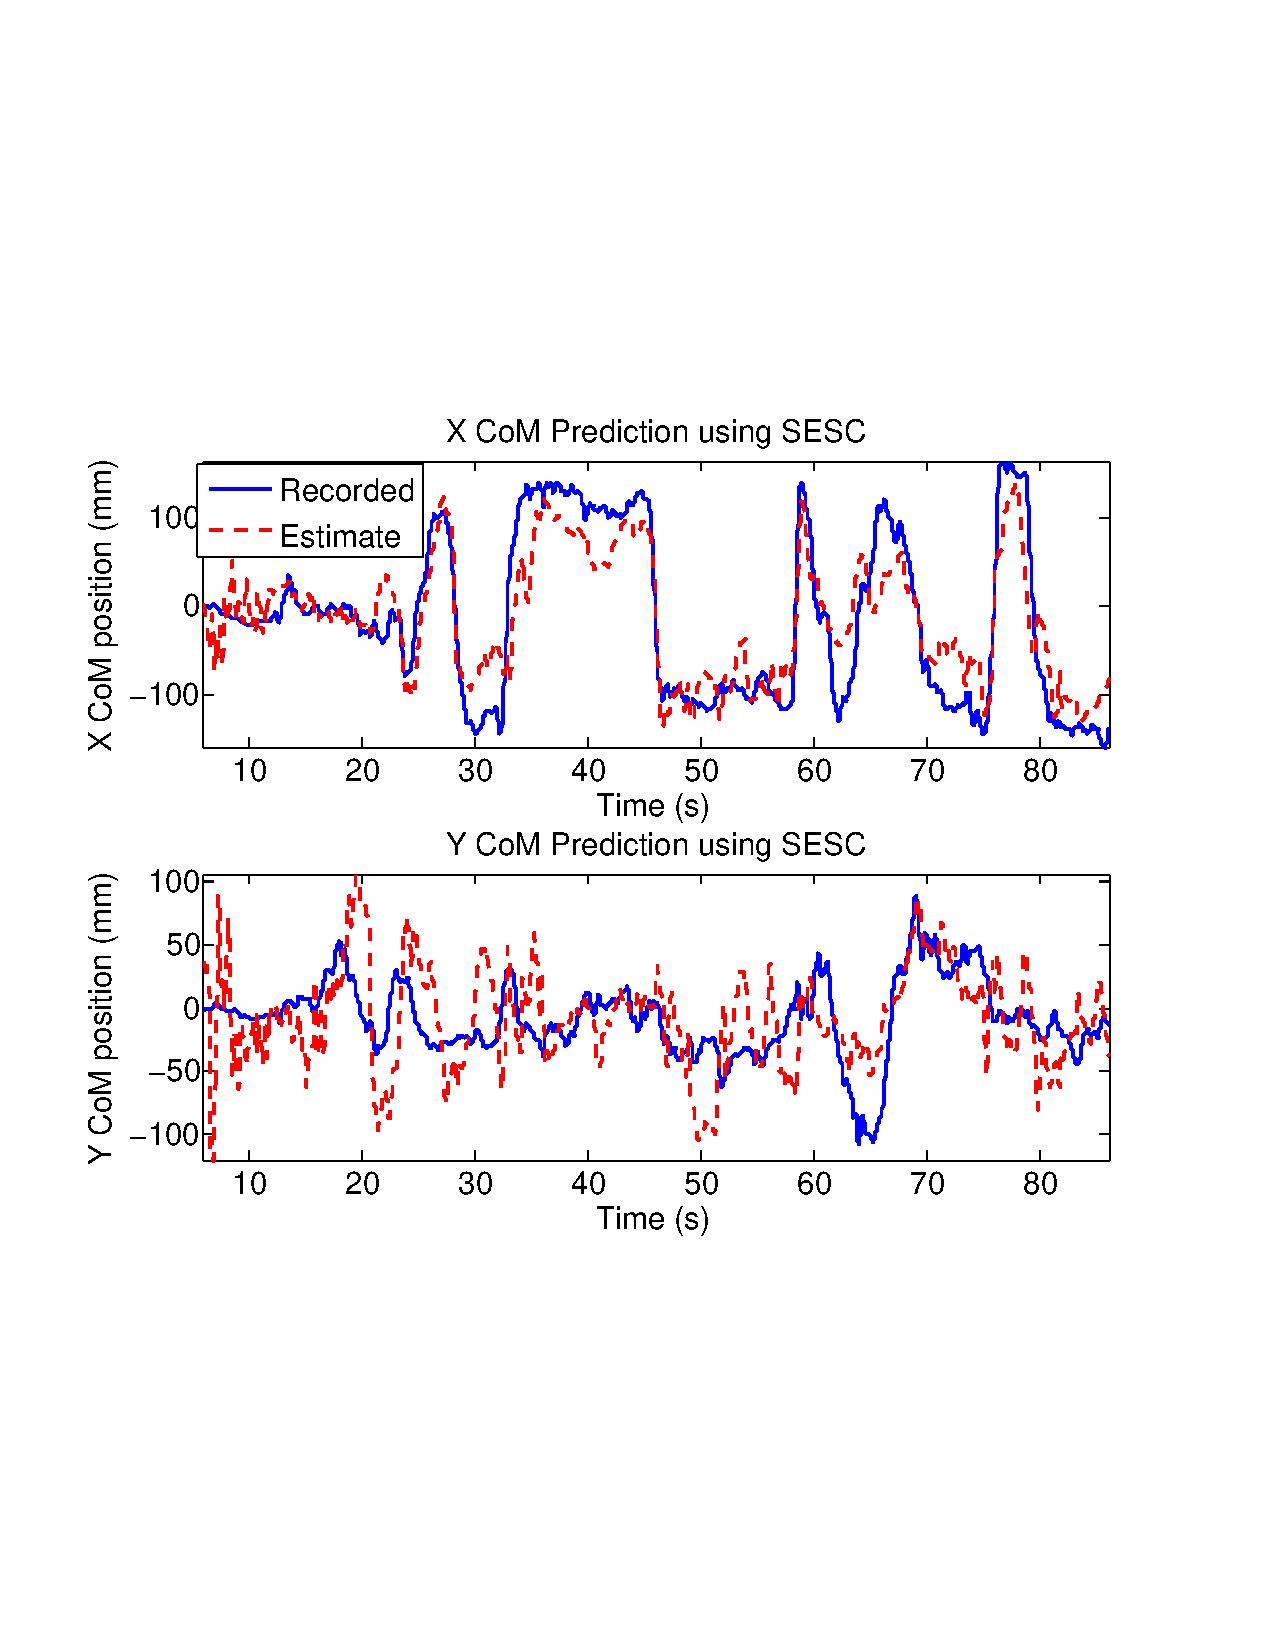
\includegraphics[trim=1cm 6cm 2cm 4cm, clip=true, width=0.6\columnwidth]{figures/SESC_Test2.pdf} 
%\end{subfigure}
%\end{tabular}
%\caption{CoM prediction using (Top) MH, (Middle) PF, (Bottom) SESC}
%\label{fig:pedestrian}
%\end{figure*}
%
%\begin{figure}
%  \centering
%    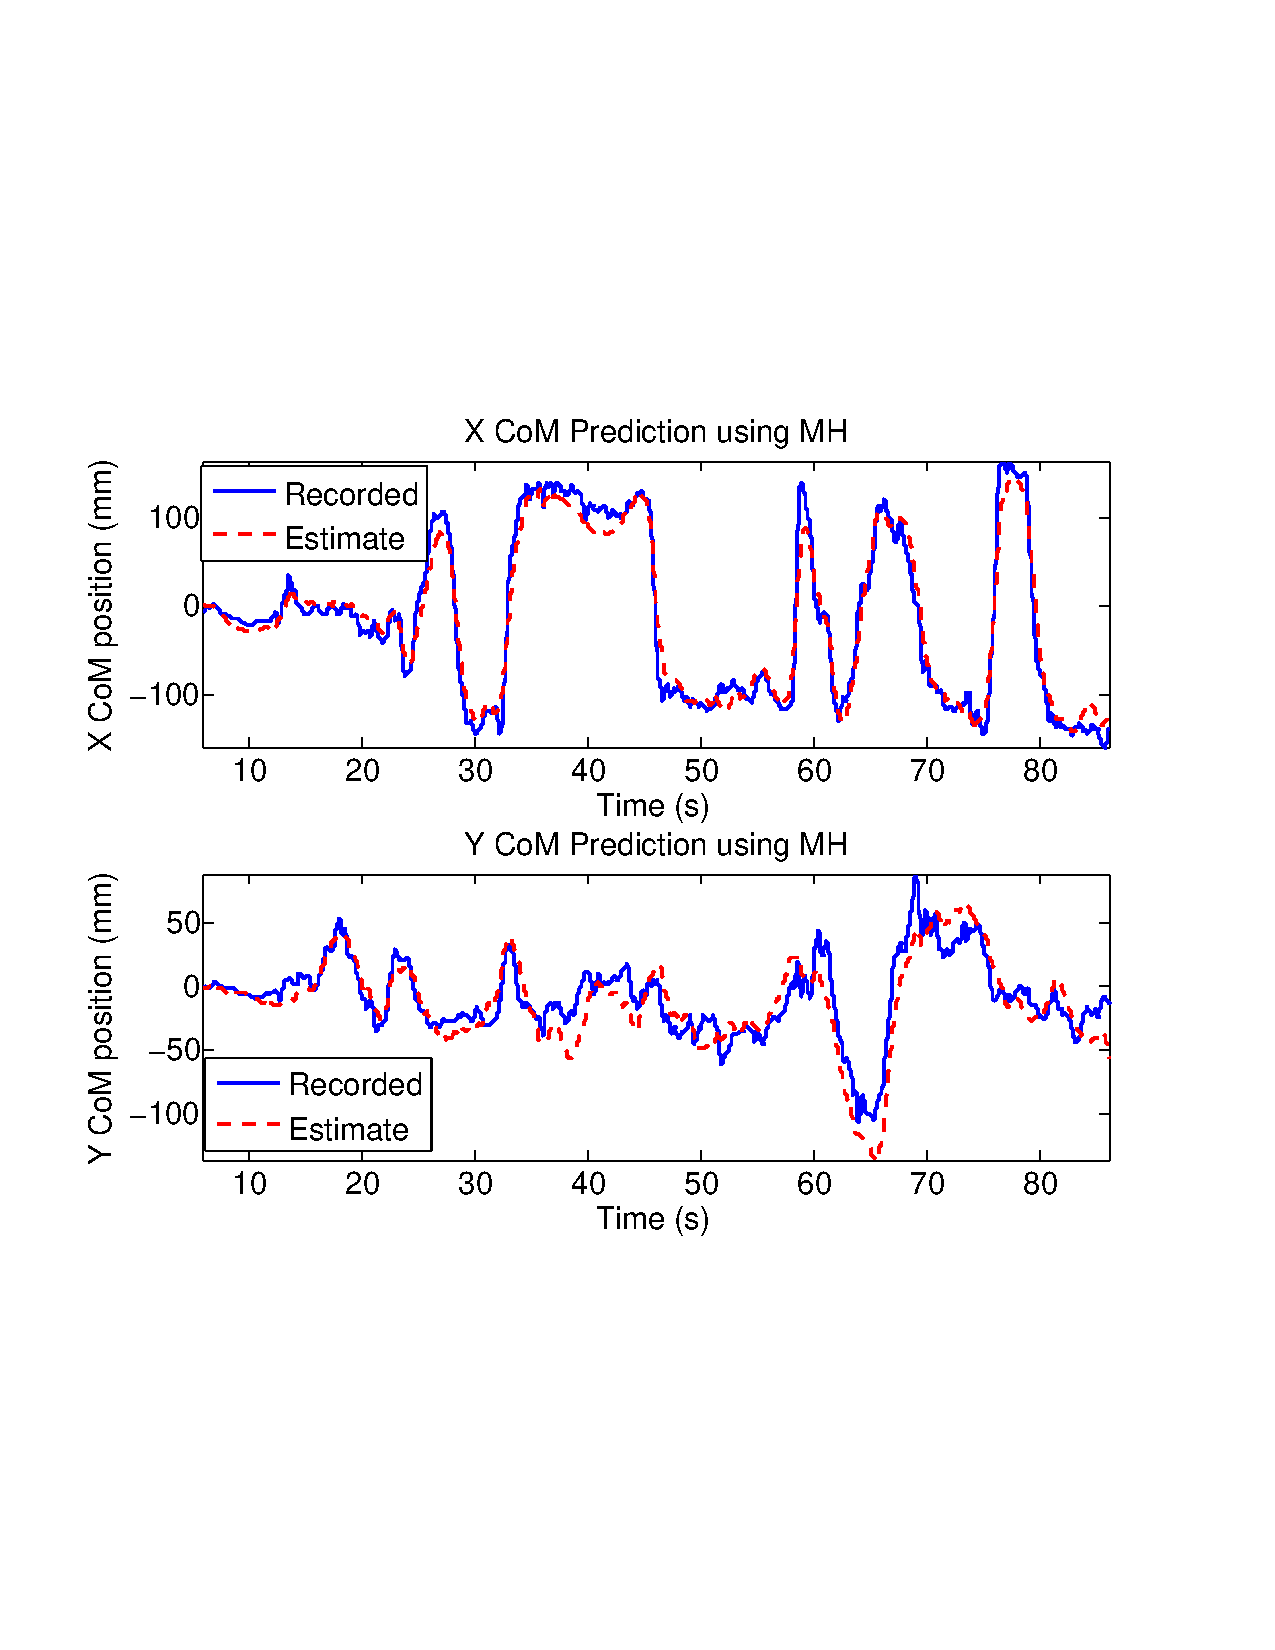
\includegraphics[trim=1cm 6cm 2cm 4cm, clip=true, width=0.9\columnwidth]{figures/MH_Test2.pdf}
%\vspace{-0.15in}
%\caption{CoM prediction using mass distribution obtained by MH }
%\label{fig:com1}
%%\vspace{-0.2in}
%\end{figure}
%
%\begin{figure}
%  \centering
%    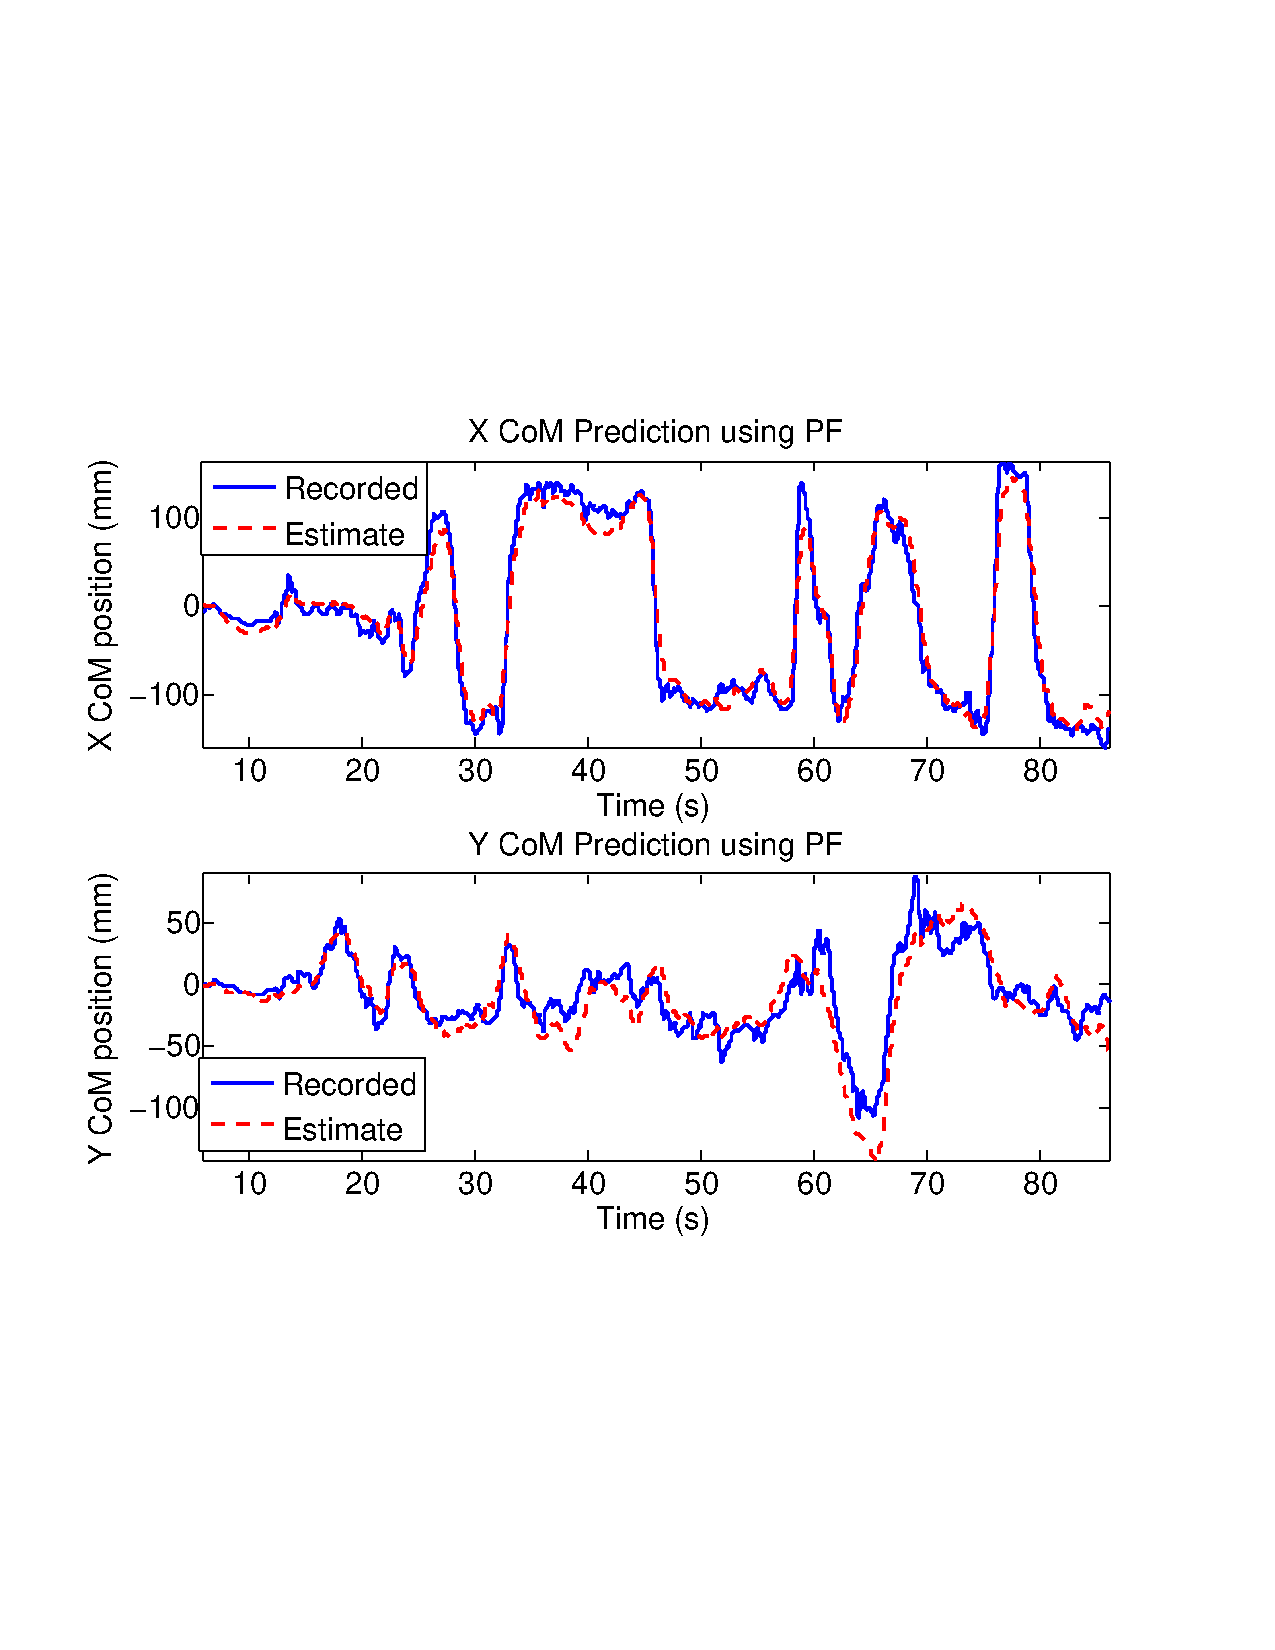
\includegraphics[trim=1cm 6cm 2cm 4cm, clip=true, width=0.9\columnwidth]{figures/PF_Test2.pdf}
%\vspace{-0.15in}
%\caption{CoM prediction using mass distribution obtained by PF }
%\label{fig:com1}
%%\vspace{-0.2in}
%\end{figure}
%
%\begin{figure}
%  \centering
%    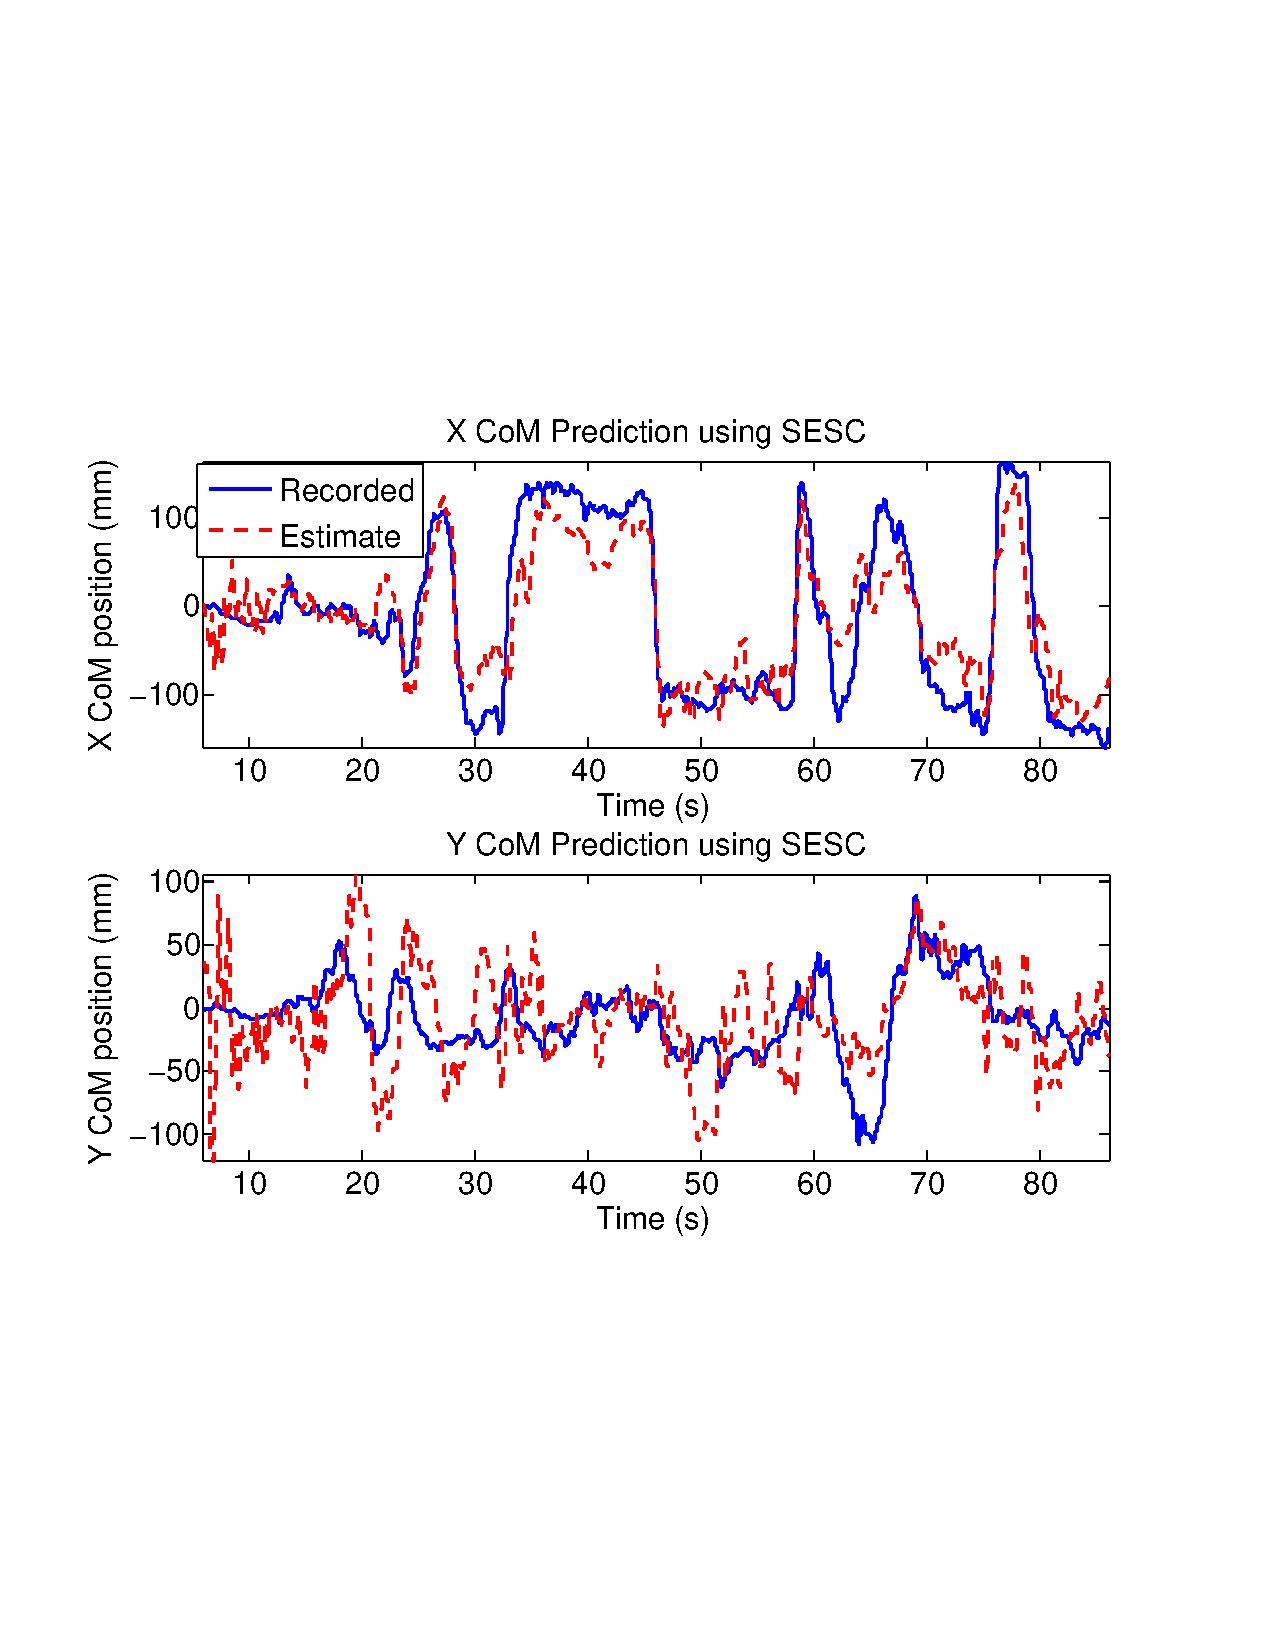
\includegraphics[trim=1cm 6cm 2cm 4cm, clip=true, width=0.9\columnwidth]{figures/SESC_Test2.pdf}
%\vspace{-0.15in}
%\caption{CoM prediction using SESC model}
%\label{fig:com1}
%%\vspace{-0.2in}
%\end{figure}
%
%
%\begin{figure}
%  \centering
%    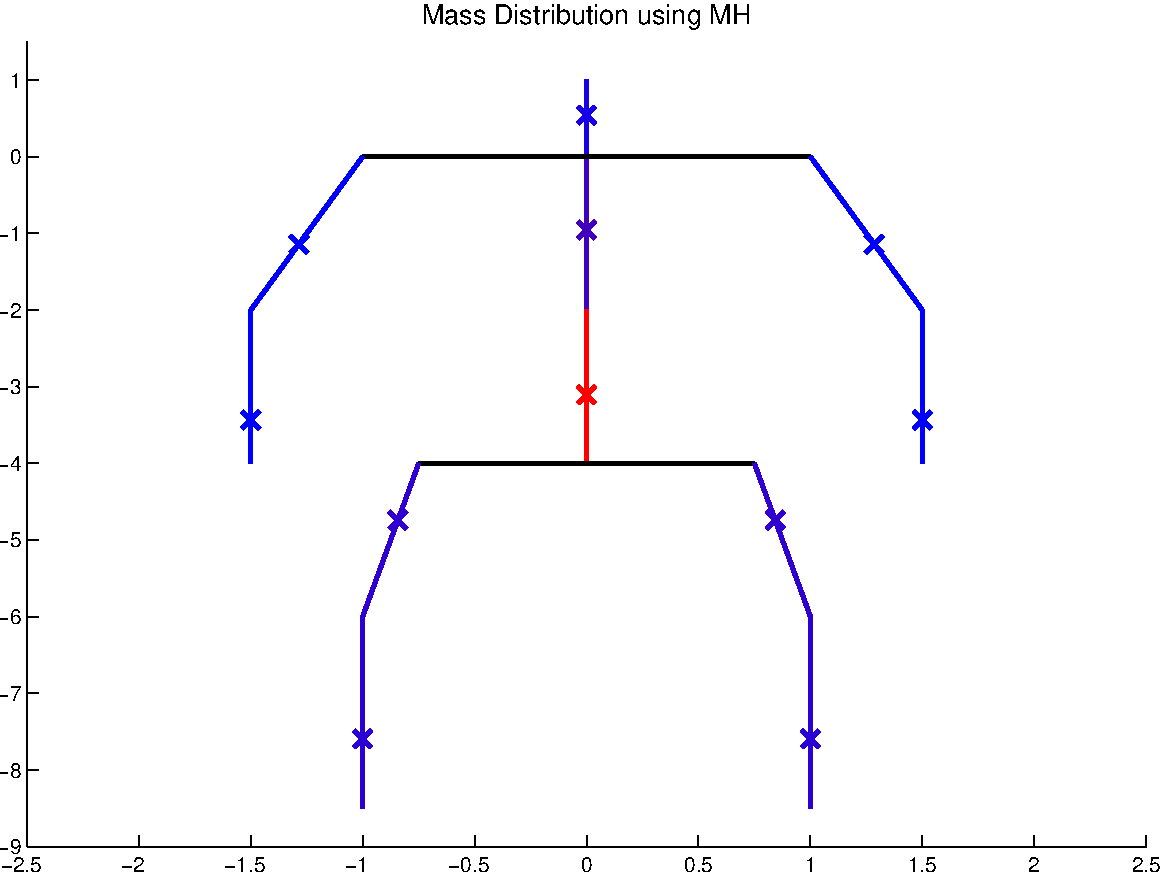
\includegraphics[width=0.85\columnwidth]{figures/Massdist_MH.pdf}
%\vspace{-0.15in}
%\caption{Mass Distribution obtained by MH }%Due to the large state space, changepoint detection and model reclassification is occassionally delayed. }
%\label{fig:com1}
%%\vspace{-0.2in}
%\end{figure}
%
%\begin{figure}
%  \centering
%    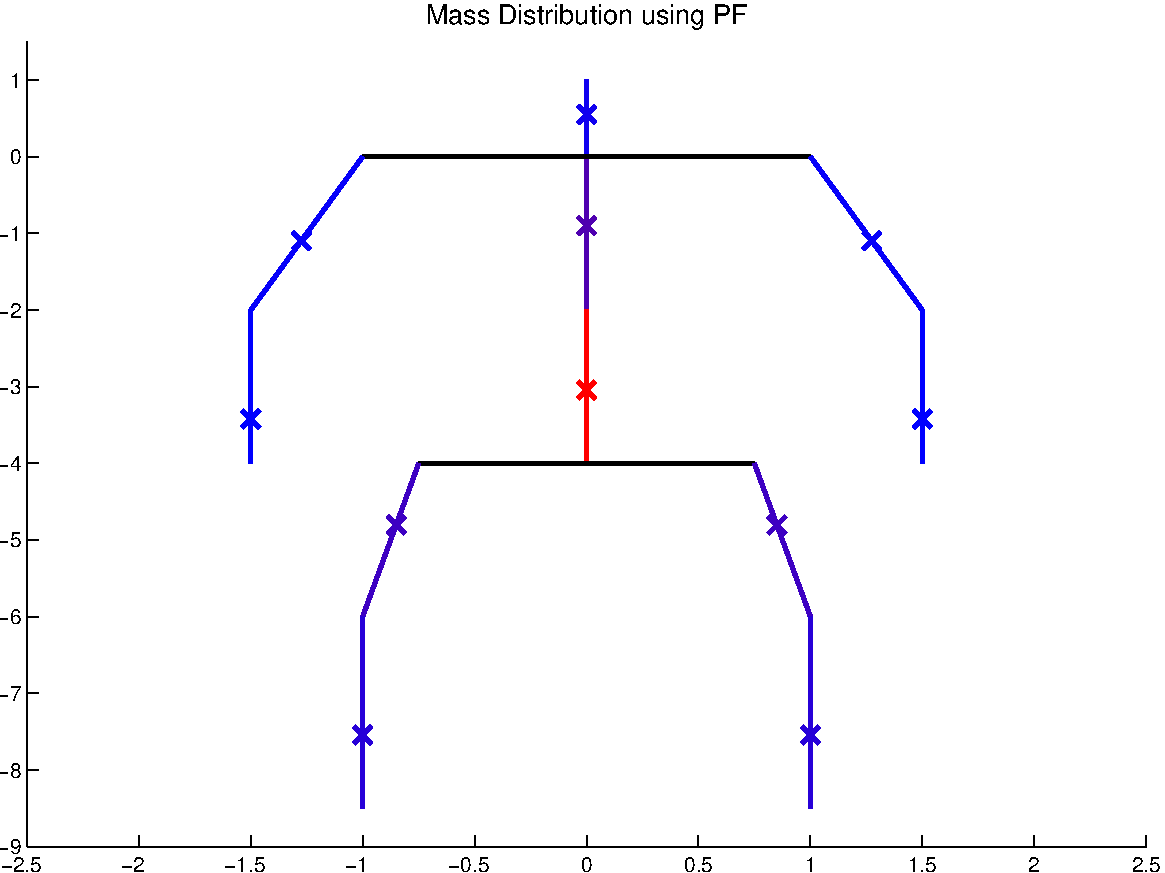
\includegraphics[width=0.85\columnwidth]{figures/Massdist_PF.pdf}
%\vspace{-0.15in}
%\caption{Mass Distribution obtained by PF}%Due to the large state space, changepoint detection and model reclassification is occassionally delayed. }
%\label{fig:com1}
%%\vspace{-0.2in}
%\end{figure}
%
%\begin{figure}
%  \centering
%    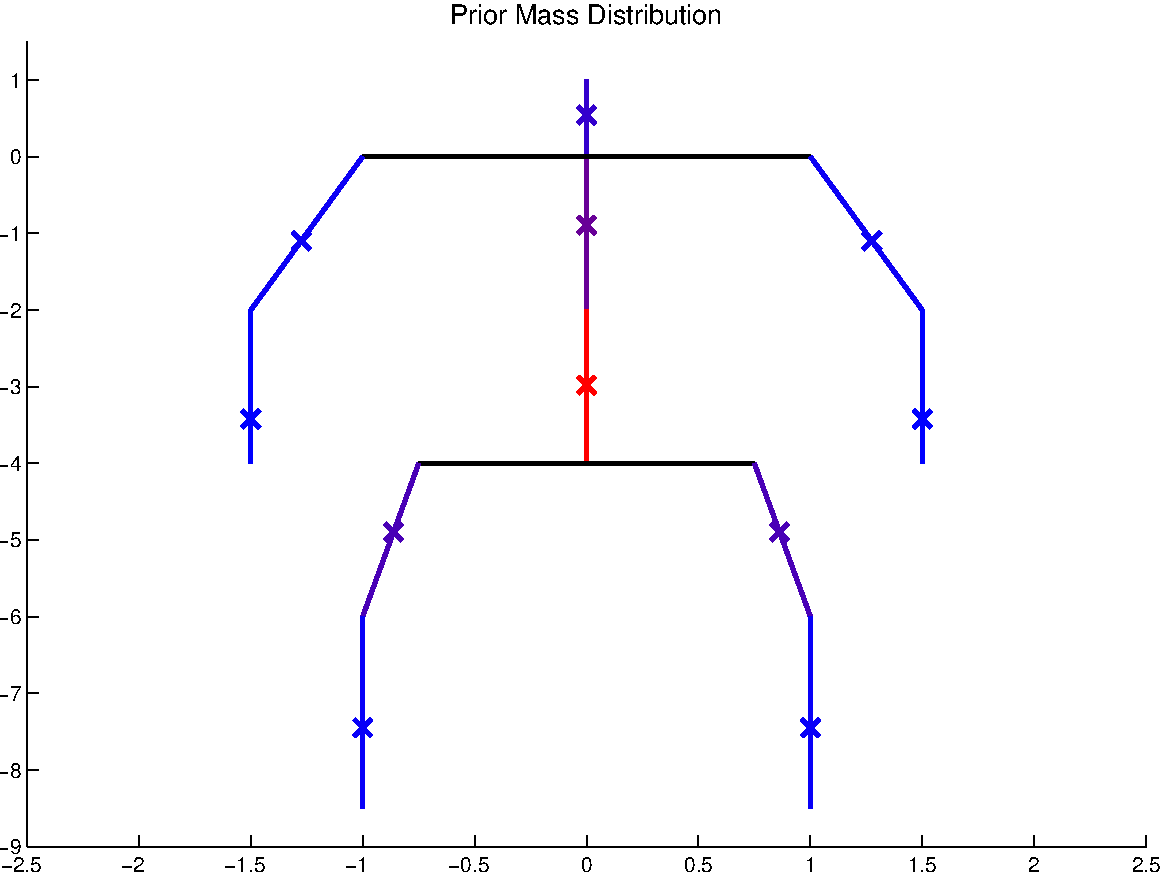
\includegraphics[width=0.85\columnwidth]{figures/Massdist_Prior.pdf}
%\vspace{-0.15in}
%\caption{Prior Mass Distribution}%Due to the large state space, changepoint detection and model reclassification is occassionally delayed. }
%\label{fig:com1}
%%\vspace{-0.2in}
%\end{figure}
%

In general, both the the PF and MH algorithms perform well in terms of predicting the CoM location. Both algorithms outperform the SESC algorithm by approximately a factor a two for all subjects. CoM predictions are generally within 30~mm of the Wii Balance Board prediction, so the prediction capability is quite reliable. On the other hand, the SESC algorithm appears to overfit the parameters and perform poorly, especially in the $y$ dimension. All algorithms had more difficulty in predicting the $y$ position of the CoM, most likely due to the fact that the Kinect sensor is not as accurate in measuring depth. 

The MH and PF algorithms return reasonable estimate for the inertial parameters, although there is some variability between the results returned by the algorithms. It is likely that a more thorough training phase is needed in which the subject performs a greater variety of movements focusing on specific limbs. For example, if a subject lifts his full arm up, the algorithm cannot distinguish the difference between the lower arm and the upper arm, because both are moving simultaneously. On the other hand, if one moves only the lower arm, keeping the upper arm fixed, this would help the algorithm find the true parameters. 



\section{DISCUSSION}
%\input{s_theory_PAC}
%\XX{what is the contribution?? make it sink home with the reviewers}
This paper presented a novel method for estimating the mass distribution of a human using a position and center of mass measurements of a human performing slow moving or static poses. 
Unlike previous methods, our setup does not require expensive or specialized equipment and only requires a Kinect and Wii Balance Board.
Using such inexpensive equipment requires that the dataset contain only slow moving or static poses in order for the measurements to be reliable. 
However, in Section \ref{prelim}, it was shown that using only static position measurements, it is impossible to determine the mass distribution due to an observability problem. 
Therefore, the problem was formulated in the Bayesian framework using prior distributions derived from the medical literature, and two approximate Bayesian inference algorithms, Metropolis-Hasting (MH) and the Particle Filter (PF), were used to estimate the mass distribution. 
In Section \ref{experiments}, it was shown that the MH and PF estimates of mass distribution were close to those in the medical literature and that using these mass distribution estimates, one can successfully predict the center of mass of a human from observed joint angles. 
Additionally, both MH and PF algorithms outperformed the Statically Equivalent Serial Chain (SESC) Model \cite{gonzalez2012estimation} in terms of prediction error of the center of mass for new test data.

Further work will focus on using these human inertial parameter estimates to allow a humanoid robot with different inertial parameters to imitate the motion of a human operator. 
Additionally, future work will focus on methods for generating feedback for users during the training phase to generate poses which result in the most uncertainty reduction.





\addtolength{\textheight}{-12cm}   % This command serves to balance the column lengths
                                  % on the last page of the document manually. It shortens
                                  % the textheight of the last page by a suitable amount.
                                  % This command does not take effect until the next page
                                  % so it should come on the page before the last. Make
                                  % sure that you do not shorten the textheight too much.

%%%%%%%%%%%%%%%%%%%%%%%%%%%%%%%%%%%%%%%%%%%%%%%%%%%%%%%%%%%%%%%%%%%%%%%%%%%%%%%%



%%%%%%%%%%%%%%%%%%%%%%%%%%%%%%%%%%%%%%%%%%%%%%%%%%%%%%%%%%%%%%%%%%%%%%%%%%%%%%%%


\section*{ACKNOWLEDGMENT}
This work was supported by the KIST Institutional Program(Project No. 2E24800).


%%%%%%%%%%%%%%%%%%%%%%%%%%%%%%%%%%%%%%%%%%%%%%%%%%%%%%%%%%%%%%%%%%%%%%%%%%%%%%%%


\bibliography{BIB_all/controls}
\bibliographystyle{IEEEtran}


\end{document}
